% The \DocumentMetadata command is used to activate LaTeX3 features
\DocumentMetadata{}
\documentclass[a4paper, 11pt]{report}

\usepackage[draft]{latexcourse}
\usepackage{tocbibind}
\makeindex

\hypersetup{href/protocol=https://}

\title{A second course in \LaTeX}
\author{Petri Laarne\\University of Helsinki}
\date{\today}


\begin{document}

\maketitle

\tableofcontents

% Each chapter is in its own file.
% This is commonly discouraged in e.g. article manuscripts,
% and might be an overkill even for a (short-ish) dissertation,
% but I personally find it easier in my workflow.
\addtocounter{chapter}{-1}
\chapter{Introduction}


These notes were created for a course called \emph{Advanced \LaTeX},
offered to PhD students at University of Helsinki in springs~2024 and~2025.%
\footnote{I dislike the name of the course.
As you will find out, we do not talk very much about advanced topics like
\TeX{} internals or package development.
A better name would be \emph{Professional \LaTeX} or \emph{A second course in \LaTeX},
as these notes are named.}
They attempt to give a somewhat unified view of what \LaTeX{} is,
how it works, and how it should be used in producing scientific literature.
They are much larger than can be covered in a two-week intensive course
-- my hope is that they can work as a reference as well.

These notes owe a lot to \emph{The \LaTeX{} Companion} \cite{TLC}
by Frank Mittelbach and other \LaTeX{} team members.
The third edition of the book is a treasure trove for a serious \LaTeX nician,
but at three kilograms (printed version) it is not an investment for everybody.
I have tried to distill some of the wisdom%
\footnote{While undoubtedly introducing some un-wisdom of my own.}
into these notes (which are still not what you'd call lightweight).

Of course, the authoritative reference for each package is the documentation hosted on
the Comprehensive \TeX{} Archive Network (\url{ctan.org}).



%
%
\section{What you need}

I assume that you already know the basics of \LaTeX{}
-- ideally, you have written a Bachelor's or Master's thesis or an article with it.

You need to have an up-to-date \LaTeX{} environment.
If you use a local installation, pause now for a moment
and check whether the packages are up to date.
If you use Overleaf, then the system is already good to go.

I encourage you to compare different editor programs.
As programmers can testify, having a good editor makes coding much more pleasant.
It is good to get familiar with the keyboard shortcuts your editor offers.

Since there are so many editors and they change much faster than base \LaTeX,
these notes do not discuss their use.

\begin{overleaf}
As an exception, there are a few blocks like this that discuss Overleaf.
I felt that Overleaf is worth mentioning, since so many people use it nowadays,
and it has some differences to locally installed tools.
\end{overleaf}


%
%
\section{About this version}

This is Version~1.1 of the notes, published at the end of the Spring~2025 course.

This version contains some fixes and additions to the 1.0~version,
but it is still in need of a good copy editor.
All red \textcolor{red}{\textbf{TODO}} notes that were there at the end of the~2024 course
have just been turned into blue \textcolor{blue}{\textbf{FUTURE}} notes,
only visible in the working draft available on GitHub (see below).

\future{Particular examples that need work are the index,
and writing everything in a more consistent tone.
Some remarks should just be deleted.
The section on tables should talk about \textsf{tabulary}.
As an internal change, there should be starred (no-index) formatting commands,
and warnings should be cleared.}

Maybe someday I will have a chance to properly polish these notes.
Any comments and suggestions are more than welcome.



%
%
\section{See how it is made}

\noindent{\Huge\faCreativeCommons\faCreativeCommonsBy}
These notes are licensed under the Creative Commons Attribution~4.0 license.%
\footnote{\url{creativecommons.org/licenses/by/4.0/}}
You are free to copy and redistribute them as you like.
You can also modify and reuse them freely,
under the condition that you indicate clearly the original author
and whether you have modified the work.
You can see the license terms for complete description.

\bigskip\noindent{\huge\faGithub}
The source code and latest PDF~release for these notes are available on GitHub:
\url{github.com/polsys/2nd-course-latex}.

You are invited to see how I built these notes
-- I tried to follow my own guidelines, but of course you can disagree with some choices.
In the end, there is no one true path to \TeX nical enlightenment.

If you spot a typo or an error, you can send a pull request with the correction,
file a GitHub issue, or send me an email about it.
You can find my up-to-date contact information at \url{petri.laarne.fi}.

\bigskip\noindent
I hope that you find these notes useful!

% !TeX root = 2nd-course-in-latex.tex
% (The appearance of \documentclass in the examples confuses LaTeX Workshop for VS Code)

\chapter{Programming}

What really is \LaTeX?

It all starts with \TeX, the typesetting system designed by Donald Knuth in late 70s and 80s.
\TeX{} is a powerful system for laying out text,
but it puts a lot of responsibility on the writer.
Essentially, you are responsible for both the content and its presentation.

\LaTeX{} (originally by Leslie Lamport, now maintained by several people)
extends this core by introducing commands like \cmd{section}:
this command not only lays out the section title in a bigger font,
but also adds some vertical whitespace around it, updates the current section number,
adds an entry to the table of contents, and so on.
This \emph{separates the content from how it is presented}.

We will try to emphasize this philosophy on this course.
By using standard constructs, packages, and our own custom commands,
we can make the \verb|.tex| source code \emph{semantically} meaningful:
something that you could read aloud.
The system then makes sure that the output looks great on paper
-- isn't that why we ever wanted computers to exist!


\begin{warning}
Even when using \LaTeX{}, the old \TeX{} is still there.
It is possible to use plain-\TeX{} commands in your documents,
but \emph{this is highly discouraged}.
These commands sidestep all the enhancements brought by \LaTeX,
and might cause hard-to-diagnose problems.
You might need them when writing more complicated packages,
but then you are already solidly in the ``you are free to shoot your own foot'' territory.
Some such commands are noted in these Warnings.

Unfortunately, many heritage templates and Stack Exchange answers still mix
\TeX{}, \LaTeX, and pre-1994 \LaTeX.
Examples of the latter include the obsolete \obscmd{em}, \obscmd{bf}, and \obscmd{it} commands
(e.g.\ writing \verb|{\bf bold}| instead of \verb|\textbf{bold}|).
\end{warning}


\begin{latexthree}
The ``standard'' \LaTeX{} version is $2\varepsilon$, released in 1994.
\LaTeX3 is a long-running project (started already before $2\varepsilon$, and reactivated around 2018)
on rewriting the internals of \LaTeX{} to be more extensible.

\LaTeX3 introduces new commands for defining commands and environments.
We will only discuss the version $2\varepsilon$ methods (which are still valid) here,
but if you find yourself writing a package, you should consider learning about the new methods.

We will talk about some new features and accessibility improvements brought by \LaTeX3 below,
starting already in \Cref{sec:document structure}.
\end{latexthree}



%
%
%
\section{Commands and environments}

\begin{practices}
When should you define your own commands?
Generally, the less customization you have,
the easier your manuscript is for the journal publication process and your coauthors.
At the same time, good commands make the code semantically meaningful.

I personally find \verb&\norm{...}& easier to read than \verb&\left\|...\right\|&,
and \verb|\Prob| certainly better than \verb|\mathbb P|,
but others could find those an overkill.
This is a hard balance to strike.

There is just one strict rule:
never repurpose the name of an existing base \LaTeX{} command.
It will cause endless trouble when some part of the journal style tries to use the original command.
\end{practices}


\subsection{Defining commands}
\index{macros}
\TeX{} is a macro language.
This means that there are special source code tokens (\emph{macros}),
that are \emph{expanded} into sequences of more tokens
(including more macros, which are expanded recursively).
The core system includes only a few commands for manipulating internal state and putting out text,
and the rest is achieved via macro expansion.

That was a mouthful, so let us see an example.
In \LaTeX{} macros are defined with the \cmd{newcommand} command.

\begin{VerbatimOut}{\jobname.tmp}
\newcommand{\hello}{Hello world!}

\hello
\end{VerbatimOut}
\ShowExample

Here \cmd{newcommand} takes two arguments:
the first is the name of the macro to define, and the second is what the macro expands to.
In \TeX{} things are grouped with the \verb|{}| braces.
(The first set of braces is technically unnecessary, but it looks cleaner in my opinion.)

Let us see another example where the command is used repeatedly,
and also expanded inside other commands:
\indexcmd{MakeUppercase}
\begin{VerbatimOut}{\jobname.tmp}
\newcommand{\hello}{Hello world}

--\hello, they whispered.\\
--I said, \MakeUppercase{\hello}!
\end{VerbatimOut}
\ShowExample

Since the macros are expanded recursively until there is nothing more to expand,
you can write things that are semantically very unclear,
but comprehensible to a computer:
\begin{VerbatimOut}{\jobname.tmp}
\newcommand{\hi}{^\infty}
\newcommand{\underscore}{_}
\newcommand{\lo}{\underscore{i=1}}

\[ \sum\lo\hi \]
\end{VerbatimOut}
\ShowExample
%
The expansion goes something like this:
\begin{enumerate}
    \item \verb|\sum\lo\hi|
    \item \verb|\sum\underscore{i=1}\hi|
    \item \verb|\sum_{i=1}\hi|
    \item \verb|\sum_{i=1}^\infty|
\end{enumerate}
So the end result is the same as if one had written the sum sensibly from the beginning.



\begin{warning}
In plain \TeX{} macros are defined with \obscmd{def} and \obscmd{let}.
If you see code using either,
you have entered the ``shoot your own foot'' territory.\footnotemark
\end{warning}
\footnotetext{Since you asked, the difference between the two is whether the contents of the macro
are expanded at usage or definition time.
Neither protects you against overwriting existing macros.}
\quiettodo{Keep these on the same page!}


%
\subsection{Arguments to commands}

To pass arguments to macros, we can indicate their number with an optional argument
between the macro name and definition.
These arguments can then be accessed in the macro definition with \verb|#1|, \verb|#2|, and so on.

\begin{VerbatimOut}{\jobname.tmp}
\newcommand{\say}[2]{#1 says ``#2''!}

\say{Petri}{Hi}
\end{VerbatimOut}
\ShowExample

Arguments are often wrapped in the \verb|{}| braces,
but it is not actually necessary -- in a very specific case.
By default, \LaTeX{} interprets a single letter or a number as an argument.
The braces extend the argument to a longer stretch.

This means that all of the following are equivalent:

\begin{VerbatimOut}{\jobname.tmp}
\[
\frac{1}{2}
= \frac 1 2
= \frac12.
\]
\end{VerbatimOut}
\ShowExample

Do note the last one -- \LaTeX{} command names can only consist of letters,
so the number 1 is not interpreted as part of the command name but an argument.
There is no requirement to separate the name and a following number.
(I do find the last example hard to read, though.)
Conversely, whitespace won't separate longer arguments; you really need the braces:

\begin{VerbatimOut}{\jobname.tmp}
\[
\frac 12 34
\neq \frac {12} {34}.
\]
\end{VerbatimOut}
\ShowExample

However, commands are interpreted as single tokens.
This happens regardless of whether the command would expand to several tokens.

\begin{VerbatimOut}{\jobname.tmp}
\newcommand{\magic}{314 159}
\[ \frac \magic \pi \]
\end{VerbatimOut}
\ShowExample

\begin{gotcha}
Some built-in macros swallow the whitespace that follows them.
If a word space is actually needed, you can feed the command an empty group \verb|{}|:
\begin{VerbatimOut}{\jobname.tmp}
\LaTeX programming\\
\LaTeX{} programming
\end{VerbatimOut}
\ShowExample
\end{gotcha}


%
\subsection{Groups and scopes}

\index{group}\index{scope}
More precisely, the braces delimit a \emph{group}.
A group is handled as a single argument to a command.
Additionally, they serve as a \emph{scope} for commands that change
how all the following text is output.
For example, the font-sizing commands like \cmd{tiny} and \cmd{Large}
affect the size of all text that follows them.
However, this effect only lasts until the group is closed with a \verb|}|.

\begin{VerbatimOut}{\jobname.tmp}
{\tiny I am small}
and I am normal
and {\Large I am large}
\end{VerbatimOut}
\ShowExample

If you forget about this and just write \cmd{tiny} without any scoping,
you will have tiny text until the end of document (or the next font size command).

\begin{VerbatimOut}{\jobname.tmp}
\tiny I am small and
{\Large I am large}
and I am tiny again
\end{VerbatimOut}
\ShowExample

There is one place where the braces do not delimit a group:
in the definition of commands.
In the following example, \verb|\mouse{Squeak}| is expanded into
\verb|\tiny Squeak| and not into \verb|{\tiny Squeak}|.
Therefore the effect persists onto the following line.
%
\begin{VerbatimOut}{\jobname.tmp}
\newcommand{\mouse}[1]{Mouse: \tiny#1.}

\mouse{Squeak}\\
I: Oops.
\end{VerbatimOut}
\ShowExample
%
The scope can be introduced here by adding \verb|{}| into the command definition:
%
\begin{VerbatimOut}{\jobname.tmp}
\newcommand{\mouse}[1]{{Mouse: \tiny#1.}}

\mouse{Squeak}\\
I: Alright.
\end{VerbatimOut}
\ShowExample

Scopes also affect things like \cmd[scope]{newcommand}:
the command \verb|\mouse| defined above only exists
within the example block, and is not accessible beyond it.
\todo{I want an optional cmd argument for subindex}



%
\subsection{Optional arguments}

Some commands also have optional arguments.
Instead of braces, these are passed within brackets \verb|[]|.
A basic example is the \cmd{sqrt} command
that produces not only square roots, but general roots:
\begin{VerbatimOut}{\jobname.tmp}
$\sqrt{7}$,
$\sqrt[3]{7}$.
\end{VerbatimOut}
\ShowExample

Another example is the optional argument to \cmd{cite} command,
which indicates a precise position within the cited work:
\verb|\cite[Page 40]{TLC}| produces \cite[Page 40]{TLC}.
(Here \verb|TLC| is the bibliography key for \emph{The \LaTeX{} Companion};
we will discuss this more in \Cref{sec:bibliography})

\begin{gotcha}
Inside an optional argument, \LaTeX{} interprets the first \verb|]| it sees as the closing bracket.
This means that if you need to use \verb|[]| \emph{inside} an optional argument
(say, as an optional argument to an inner command), you need to wrap things in braces.
Quite often, you might need even \emph{two sets of braces}.
Compare the two citations:
%
\begin{VerbatimOut}{\jobname.tmp}
\cite[{{Page [40] maybe?}}]{TLC}\\
\cite[Page [40] maybe?]{TLC}
\end{VerbatimOut}
\ShowExample
%
The first citation is shown correctly.
In the second, the optional argument is interpreted to be ``\verb|Page [40|''
and the citation name then ``\verb|m|'' (only a single letter since it was not wrapped in braces).
The remaining ``\verb|aybe?]{TLC}|'' is then normal body text.
\end{gotcha}

\begin{gotcha}
\LaTeX{} ignores whitespace between a command and its optional argument.
This might sometimes lead to surprising behaviour.
Here the second list item is interpreted as an optional argument that replaces the bullet symbol:
\indexcmd{item}
%
\begin{VerbatimOut}{\jobname.tmp}
\begin{itemize}
\item Cookies
\item [Maybe cake?]
\item Drinks
\end{itemize}
\end{VerbatimOut}
\ShowExample
\end{gotcha}


The syntax for optional arguments is not always clear:
sometimes they precede the real arguments, sometimes they follow them.
Sometimes they consist of just one thing,
sometimes they can be a list of things
(see the discussion of \cmd{usepackage} later in this chapter).

\todo{Defining commands with optional arguments?}


%
\subsection{Replacing existing commands}

Sometimes it is useful to overwrite an existing command.
One common example is rewriting \cmd{epsilon} to actually mean \cmd{varepsilon},
since many consider the variant $\varepsilon$ prettier than the regular $\epsilon$.

It is not possible to write \verb|\newcommand{\epsilon}{\varepsilon}|,
since \LaTeX{} rightly complains about \verb|\epsilon| being already defined.
You could be accidentally overwriting a command used elsewhere in the document.
You have to make your intentions clear by using \cmd{renewcommand}:

\begin{VerbatimOut}{\jobname.tmp}
Old epsilon: $\epsilon$,\\
\renewcommand{\epsilon}{\varepsilon}
New epsilon: $\epsilon$.
\end{VerbatimOut}
\ShowExample
%
Again, the redefinition of a command lasts only for the current scope.
Once the scope is closed, \verb|\epsilon| again means the old regular symbol.
To redefine a command within the entire document,
you need to call \cmd{renewcommand} in the document preamble.

Here is an example of \cmd{newcommand} and \cmd{renewcommand} with arguments.
The two commands have matching syntax.
Note that the new definition is free to have a different number of arguments.

\begin{VerbatimOut}{\jobname.tmp}
\newcommand{\dual}[2]{(#1 \mid #2)}
Mathematicians: $\dual{a}{b}$.\\
\renewcommand{\dual}[2]
  {\langle#2 \mid #1\rangle}
Physicists: $\dual{a}{b}$.
\end{VerbatimOut}
\ShowExample


\todo{Advanced: adding to an existing command.}


%
\subsection{Defining environments}

\index{environments}
Environments encapsulate larger blocks of text.
They also form implicit groups.

\begin{VerbatimOut}{\jobname.tmp}
\begin{center}
\renewcommand{\epsilon}{\varepsilon}
Centered text and $\epsilon$
\end{center}

\begin{flushright}
Right-aligned text.
Here we have the old $\epsilon$.
\end{flushright}
\end{VerbatimOut}
\ShowExample

To define an environment, we use the \cmd{newenvironment} command.
This command takes three arguments: the name of the environment
and code to expand at the beginning and the end of the environment.

\begin{VerbatimOut}{\jobname.tmp}
\newenvironment{cool}
    {A mathmo enters the lab.\par}
    {\par The mathmo leaves the lab.}

\begin{cool}
A massive explosion occurs.
\end{cool}
\end{VerbatimOut}
\ShowExample
%
(If you're wondering about the \cmd{par} commands,
they are used to ensure that the first and last lines are their own paragraphs.)

There is also \cmd{renewenvironment} that works like \verb|\renewcommand|.

Since environments are groups,
it is possible to change font characteristics for the duration of the environment:

\begin{VerbatimOut}{\jobname.tmp}
\newenvironment{mouse}{\tiny}{}

Ordinary text.
\begin{mouse}
Very small and very squeaky text.
\end{mouse}
Again ordinary text.
\end{VerbatimOut}
\ShowExample
%
Note that here the end code is empty;
the font properties are reset automatically as the group ends.

\begin{gotcha}
If the begin/end code of your environment spans multiple lines,
you need to be careful with line breaks.
The extra whitespace might cause \LaTeX{} to output an unintended empty space
or even a paragraph break.
To avoid line breaks to be interpreted as line breaks,
you can end each line in the environment definition with \verb|%|
-- the comment character shallows the line break.

This same thing applies to empty lines before and after environment usage
-- the usual paragraph-breaking rules apply.
If you don't want to start a new paragraph after the environment ends,
do not leave an empty line between \verb|\end{...}| and the following text.
(For visual separation in the code, I prefer a line containing just \verb|%|.)
\end{gotcha}



\todo{Parameter form; improvements in L3}


%
%
%
\section{Diagnosing errors}

Macro languages were popular in the 1980s, back when 640 kilobytes was enough memory for anyone.
An unfortunate consequence of \TeX's stability is that the compiler still operates under this worldview.
The source code is read exactly once from top to bottom,
and if the code is not correct, error messages can be extremely cryptic.

\begin{overleaf}
Some \LaTeX{} distributions are set up to ignore some errors.
For example, Overleaf is quite good at ignoring missing \verb|$| signs and other small typos.
You should really pay attention to red symbols in the source code margin
and next to the \emph{Recompile} button!
\end{overleaf}

\todo{Understanding error messages}



%
%
%
\section{Document structure}\label{sec:document structure}

Let us then look at the basic structure of a \verb|.tex| file.
Everyone reading these notes is assumed to have seen such a file more than once,
but we will spend some time on some nuances.
Bear with me even if this sounds trivial!

\begin{practices}
I would advocate for starting every project from a minimal \verb|.tex| file, like the one below.
The problem with ``heritage'' templates is that they accumulate a lot
of unnecessary package dependencies and custom commands.
I've seen files where the same package is loaded three times.

By starting from an empty file
and only adding the customizations you need for the particular project,
you help maintain your ``code hygiene''.
\end{practices}

Let us start with the minimal example below.

\begin{ExampleCode}[numbers=left]
\documentclass[a4paper]{article}

\usepackage[hidelinks]{hyperref}

\title{My first document}
\author{Firstname Lastname}
\date{\today}

\begin{document}

\maketitle

% Rest of content here...

\end{document}
\end{ExampleCode}

On the first line, we load a \LaTeX{} document class.
The document class determines the basic layout of your document,
and it is where several basic commands like \cmd{maketitle} are defined.
We will look at some different document classes and arguments in the next subsection.

Lines 1--8 are collectively known as the \emph{preamble}.\index{preamble}
This is the best place to define new commands and do other setup.
Additional packages are also loaded here; see \Cref{sec:loading packages}.

Trying to output any text before the \verb|\begin{document}| line is an error.
\indexenv{document}%
When the compiler reaches that line,
a lot of stuff happens behind the scenes to prepare \LaTeX{} for actually outputting pages.

Similarly, the \verb|\end{document}| line is necessary.
At that point, a lot of code is executed to make sure that everything is output properly.
Any text written below that line is ignored.
(I do not recommend writing anything there!)

\begin{latexthree}
An important part of the \LaTeX3 project is revising the PDF output
to include accessibility information:
for example, tagging section headings as headings and not just bold text in big font.
Since this might cause issues with some packages, the new behaviour is opt-in.

If you write \indexcmd{DocumentMetadata}\verb|DocumentMetadata{}|
before the \verb|\documentclass| declaration, you opt in to these new features.
This command also enables new functionality in e.g.\ the \pkg{hyperref} package.
\end{latexthree}


%
\subsection{Document classes}

\begin{practices}
Journals commonly define their own document classes, based on one of the standard classes.
The discussion below only applies to the documents where you are in charge of the style.
Always look at the journal instructions for preparing the published version of your article.
\end{practices}

\index{document classes}
There are three document classes of interest included in base \LaTeX{}:

\begin{description}
\item[article] As the name suggests, this should be used for articles, short notes, and such.
    The \cmd{maketitle} command does not create a separate title page,
    and the highest-level sectioning command is \cmd{section}.
    There is no page break between sections.
\item[report] This class is suitable for e.g.\ a thesis, lecture notes, or a longer article.
    The present notes use this class.
    There is a separate title page,
    and the highest-level sectioning command is \cmd{chapter}.
    Each chapter begins on a new page.
\item[book] This is the heaviest of all the classes.
    You get a lot of empty pages, just like in a real printed book.
    If you find yourself using this class,
    you have agreed to something monumental.
\end{description}
%
There is also a \textbf{letter} document class,
which understandably sees little use nowadays.
But it is still there if you need it!

Options passed to document classes are interesting in that
\emph{they are also passed to all packages}.
If you pass \verb|a4paper| to the document class (as you should),
then you don't need to pass it again to the \pkg{geometry} package.

Some options are supported by all the basic document classes:

\begin{description}
\item[a4paper] This is self-explanatory.
    By default, \LaTeX{} assumes the American letter paper size.
\item[a5paper] At least University of Helsinki uses A5 as the thesis format.
\item[10pt, 11pt, 12pt] Sets the body font size.
    Fonts for section headers, footnotes, etc.\ are scaled accordingly.
    The default is 10~points.
\item[oneside, twoside] Whether the margins are equal
    or alternating between odd and even pages.
    For example this document (which is aimed for consuption on a screen)
    uses \verb|oneside|, but a printed report should specify \verb|twoside|.
\item[openright, openany]
    Whether chapters always begin on a right-hand side page (default for book)
    or any page (default for report).
    You should consider \verb|openright| for a printed thesis.
    Not applicable to the article class where chapters are not supported at all.
\item[notitlepage, titlepage] Whether the title is set on a separate page.
\item[fleqn] Instead of centering, left-aligns display formulas.
\item[twocolumn] Sets the text in two columns.
\end{description}


A very common alternative document class is \textbf{amsart}.\indexpkg{amsart}
It is developed by the American Mathematical Society,
and some prefer its style to that of \textbf{article}.
It is a drop-in replacement for \textbf{article} and supports the same options.

Other common classes include those from \pkg{koma-script}
(drop-in replacements for all standard classes)
and \pkg{memoir} (intended for longer documents),
which both provide a lot of flexibility.
They both come with extensive documentation for those who wish to venture into that rabbit hole.


%
\subsection{Loading packages}\label{sec:loading packages}

In the previous example, we loaded the \pkg{hyperref} package with:
\begin{ExampleCode}
\usepackage[hidelinks]{hyperref}
\end{ExampleCode}
Options can be passed to packages inside the brackets.
Here we pass the \verb|hidelinks| option that suppresses the coloured boxes around clickable links.
Some packages also take options with a \verb|key=value| notation.

In addition to the options passed explicitly,
all the options passed to the document class are also forwarded to the package.

\begin{practices}
You should always load \pkg{hyperref}.
It not only turns cross-references into clickable links,
but also adds section headers to the PDF table of contents
(usually found in the sidebar of any reader application).
Your readers will appreciate this navigation aid.
\end{practices}

\index{packages!finding}
CTAN, the \emph{Comprehensive \TeX{} Archive Network},
is the repository for \LaTeX{} packages.
It can be browsed at \url{www.ctan.org}.

Generally \LaTeX{} distributions either contain the whole CTAN,
or are able to download packages from there as needed.
You should check out how you can keep your distribution up to date,
as new versions of packages are continually released.

Most importantly, all major packages listed on CTAN have good documentation there.
The documentation typically includes usage examples, a complete reference,
and possible compatibility issues with other packages.
For example, you can find the (very extensive!) documentation of \pkg{hyperref}
at \url{www.ctan.org/pkg/hyperref}.

\todo{Other common packages}


\begin{gotcha}\index{packages!loading order}
Quite a few packages modify the standard \LaTeX{} commands
and even the commands defined by each other.
This means that sometimes it is important to load packages in the correct order,
so that the modifications are applied sensibly.
The core packages are usually compatible with each other,
but you should always check the package documentation for possible conflicts.

For example, it is important to load \pkg{ntheorem} before \pkg{hyperref},
since the former modifies the label commands that are also touched by the latter.
Otherwise, you might get non-functioning hyperlinks.
\end{gotcha}



\section{Creating your own style file}



%
%
%
\section{Counters}

\LaTeX{} keeps a lot of internal state in variables called \emph{counters}\index{counters}.

\begin{VerbatimOut}{\jobname.tmp}
We are in Chapter~\arabic{chapter}
and its Section~\arabic{section}.

\begin{enumerate}
\item This is item~\arabic{enumi}.
\item This is item~\arabic{enumi}.
  \begin{enumerate}
  \item Subitem~\arabic{enumii}.
  \item Subitem~\arabic{enumii}.
  \end{enumerate}
\end{enumerate}
\end{VerbatimOut}
\ShowExample

The counters seen in the above example are automatically stepped by the sectioning and list commands.
They can be manually manipulated with the \cmd{setcounter} command.
One such example is seen in Väisälä's topology textbook:

\begin{ExampleCode}
\setcounter{chapter}{-1}
\chapter{Prerequisites}

% The chapter name is printed as "0. Prerequisites"
% Note: the counter is set to -1 to compensate for \chapter stepping it
\end{ExampleCode}

It is also possible to add/subtract a value to a counter:
\indexcmd{stepcounter}\indexcmd{addtocounter}%
\begin{VerbatimOut}{\jobname.tmp}
\begin{enumerate}
\item Add one and step:
  \stepcounter{enumi}
\item Add seven and step:
  \addtocounter{enumi}{7}
\item Minus one + step:
  \addtocounter{enumi}{-1}
\item Same as above!
\end{enumerate}
\end{VerbatimOut}
\ShowExample

There are many ways to output the value of a counter:\index{counters!displaying}
%
\begin{VerbatimOut}{\jobname.tmp}
Section~\arabic{section}\\
Section~\alph{section}\\
Section~\Alph{section}\\
Section~\Roman{section}\\
Section~\fnsymbol{section}
\end{VerbatimOut}
\ShowExample
The last command \verb|\fnsymbol| is used for footnote symbols.
Note that the letter-based styles can be capitalized
by using \verb|\Roman| instead of \verb|\roman| etc.

To define your own counters, you can use \cmd{newcounter}:
\index{counters!defining}%
%
\begin{VerbatimOut}{\jobname.tmp}
\newcounter{fact}
\newcommand{\axiom}[1]{\stepcounter{fact}%
    \textbf{Rule \arabic{fact}.} #1\par}

\axiom{Don't use plain \TeX.}
\axiom{See the above.}
\end{VerbatimOut}
\ShowExample

If you want the counter to reset when another counter is stepped,
you can pass an optional argument to \cmd{newcounter}.
An example use case is to reset the counter every time a new section is started
(in which case the optional argument would be \verb|[section]|).
%
\begin{VerbatimOut}{\jobname.tmp}
\setcounter{fact}{0}
\newcommand{\axiom}[1]{\stepcounter{fact}%
    \textbf{Rule \arabic{fact}.} #1\par}
\newcounter{exc}[fact]
\newcommand{\except}[1]{\stepcounter{exc}%
  {\tiny Exception~\roman{exc}. #1}\par}

\axiom{Don't use plain \TeX.}
\except{Unless Don Knuth passes by.}
\except{Or you're a masochist.}
\axiom{See the above.}
\except{No exceptions.}
\end{VerbatimOut}
\ShowExample[4]

\begin{gotcha}
This only sees the effect of \verb|\stepcounter| on the another counter;
if you use \verb|\setcounter| to change it, the dependent counter is not reset.
\end{gotcha}

\begin{technote}
Counters are always in a global scope.\index{scope!counters}
That is, the definition of a counter does not disappear as the group is closed.
If you would like to use the same counter name again in a later context,
you can (or rather, must) reset and reuse the previous counter.

Due to this, you should probably define your counters in the preamble.
\end{technote}


%
%
%
\section{\emph{Further topics*}}

\todo{Say something about robustness}

\todo{ifthen, loops, ?}

\todo{Adding options to own packages}



\chapter{Page layout and whitespace}

\section{Units of measure and whitespace}

\todo{Inter-word spacing}

\section{Page geometry}

\todo{Landscape pages}


\section{Paragraph alignment}

\section{Headers and footers}

\section{Titles}

\chapter{Mathematics layout}\label{sec:mathematics}

Plain \TeX{} already provides a lot of facilities for typesetting mathematics,
and this is further extended by \LaTeX{} and the \pkg{amsmath} packages.
The \pkg{amsmath} package is essentially as old as \LaTeX{}.
It is automatically loaded by the Americal Mathematical Society document classes like \verb|amsart|,
so you might not even need to load it.

The package works well but has not been significantly updated since the nineties.
Some additions and bug fixes are collected in the \pkg{mathtools} package.
If you use a non-AMS document class, you can load \pkg{mathtools} instead of \pkg{amsmath}
to get slightly improved typesetting.

\begin{technote}
The \pkg{amsmath} package used to be tied to the AMS document classes,
but it is nowadays maintained by the \LaTeX{} core team.
It is one of the packages guaranteed to be present on every \LaTeX{} distribution.
\end{technote}


%
%
%
\section{Equation environments}

Standard \LaTeX{} provides the \verb|\[ ... \]| syntax for
creating a mathematics display (as opposed to inline mathematics with \verb|$ ... $|).
This environment does not support equation numbering or line breaks;
for those, \pkg{amsmath} provides a lot of options.

\begin{warning}
Plain \TeX{} used the \verb|$$ ... $$| syntax for display mathematics.
Do not use it -- the \LaTeX-style environment has some hooks and accessibility features
that the \TeX{} syntax does not have.
\end{warning}


%
%
\subsection{Single numbered equation}

The basic equation environment of \pkg{amsmath} is \env{equation}.
It sets its contents on a single line and numbers the equation:
%
\begin{VerbatimOut}{\jobname.tmp}
\begin{equation}
i \partial_t u - \Delta u = -u^3.
\end{equation}
\end{VerbatimOut}
\ShowExample

If you'd rather have an unnumbered equation,
you can use the \verb|equation*| environment.
It is essentially equivalent to \verb|\[ \]| of \LaTeX.

To customize the equation number, you can use the \cmd{tag} command.
%
\begin{VerbatimOut}{\jobname.tmp}
\begin{equation}
i \partial_t u - \Delta u = -u^3.
\tag{NLS}
\end{equation}
\end{VerbatimOut}
\ShowExample
%
The tag also appears in cross-references to this equation.
The tag is read in text mode, so any mathematical symbols need to be wrapped with \verb|$|.

If you want to change whether equations are numbered globally or per section,
use the \cmd{numberwithin} mechanism described in \Cref{sec:counters}:
%
\begin{ExampleCode}
\numberwithin{equation}{section}
\end{ExampleCode}


%
%
\subsection{Single equation on many lines}\label{sec:math split}

You can break a long expression into multiple lines with the \env{multline} environment.
Only one equation number is produced (none if you use \verb|multline*|).
Line breaks are specified with \verb|\\|:
%
\begin{VerbatimOut}{\jobname.tmp}
\begin{multline}
a^5 + 5 a^4 b \\
+ 10 a^3 b^2 + 10 a^2 b^3\\
+ 5 a b^4 + b^5
\end{multline}
\end{VerbatimOut}
\ShowExample
%
The first line is left-aligned, the last line is right-aligned,
and the rest are centered.

If you need to control the alignment,
you can use the \env{split} environment.
This environment needs to be put inside \verb|equation| (or \verb|equation*|).
The alignment point is denoted by \verb|&|:
%
\begin{VerbatimOut}{\jobname.tmp}
\begin{equation}
\begin{split}
(a+b)^2
&= (a+b)(a+b)\\
&= a^2 + 2ab + b^2.
\end{split}
\end{equation}
\end{VerbatimOut}
\ShowExample

Sometimes, you need to align with things that are not really there.
Let us produce a slightly different version of the previous example:
%
\begin{VerbatimOut}{\jobname.tmp}
\begin{equation}
\begin{split}
&\mathrel{\phantom{=}} (a+b)^2\\
&= (a+b)(a+b)\\
&= a^2 + 2ab + b^2.
\end{split}
\end{equation}
\end{VerbatimOut}
\ShowExample
%
The \cmd{phantom} command reserves enough space on the first line for $=$,
even though it is not printed there;
the \cmd{mathrel} command ensures that the spacing is that surrounding $=$ as well.
This ensures that the expressions are aligned.
The same effect can not be attained with moving the alignment symbol,
since the \TeX{} spacing algorithm (described below) cannot see across the \verb|&|:
%
\begin{VerbatimOut}{\jobname.tmp}
Bad spacing after $=$ sign:
\begin{equation}
\begin{split}
&(a+b)^2\\
= &(a+b)(a+b)\\
= &a^2 + 2ab + b^2.
\end{split}
\end{equation}
\end{VerbatimOut}
\ShowExample



%
%
\subsection{Many equations, many lines}

The \env{gather} environment collects equations, each centered.
%
\begin{VerbatimOut}{\jobname.tmp}
\begin{gather}
(a+b)^2 = a^2 + 2ab + b^2,\\
a^2 - b^2 = (a+b)(a-b).
\end{gather}
\end{VerbatimOut}
\ShowExample

This environment also supports \env{split} on one or more sub-equations:
%
\begin{VerbatimOut}{\jobname.tmp}
\begin{gather}
(a+b)^2 = a^2 + 2ab + b^2,\\
\begin{split}
(a+b)^3 &= a^3\\
&\mathrel{\phantom{=}} + 3a^2 b + 3ab^2 + b^3.
\end{split}
\end{gather}
\end{VerbatimOut}
\ShowExampleBelow

You can customize the tag of each individual equation with \cmd{tag},
and also suppress an individual tag with \cmd{notag}.
These commands can appear anywhere before the \verb|\\| that ends the particular equation.
Again, the \verb|gather*| environment suppresses all tags
except those explicitly created with \cmd{tag}.
%
\begin{VerbatimOut}{\jobname.tmp}
\begin{gather}
(a+b)^2 = a^2 + 2ab + b^2,\\
(a+b)^3 = a^3 + 3a^2 b + 3a b^2 + b^3, \notag\\
a^2 - b^2 = (a+b)(a-b). \tag{$\ast$}
\end{gather}
\end{VerbatimOut}
\ShowExampleBelow

If you need to have several aligned equations, you can use the \env{align} environment.
In comparison to \env{split}, each line is now numbered individually:
%
\begin{VerbatimOut}{\jobname.tmp}
\begin{align}
(a+b)^2
&= (a+b)(a+b)\\
&= a^2 + 2ab + b^2.
\end{align}
\end{VerbatimOut}
\ShowExample
The same remarks about \cmd{tag} and \cmd{notag} with \verb|gather| apply here.
The \env{align} environment also supports more than one alignment point.


\begin{warning}
There is also an \obsenv{eqnarray} environment provided by base \LaTeX.
It is far less sophisticated and generally uglier than
anything you can achieve with the environments presented here,
so I would avoid it.
\end{warning}

If you want to number the equations as subequations,
it can be done by wrapping the environment inside \env{subequations}:
%
\begin{VerbatimOut}{\jobname.tmp}
\begin{subequations}  
  \begin{align}
    (a+b)^2
    &= (a+b)(a+b)\\
    &= a^2 + 2ab + b^2.
  \end{align}
\end{subequations}
\end{VerbatimOut}
\ShowExample


If your equation environment is very long,
it might be beneficial to allow page breaks.
The display environments presented here do not allow page breaks by default.
By putting a \cmd{displaybreak} command before the \verb|\\|,
you indicate that a page break \emph{is allowed}.

The \cmd{allowdisplaybreaks} command permits page breaks in displays everywhere in its scope.
If you put it inside an environment, it applies to that environment only;
if you put it in the preamble, it applies to all environments.


%
%
\subsection{Cases}

To group several expressions with vertical brackets,
you can use the \env{cases} environment inside an equation environment.
This environment supports a single alignment \verb|&|:
%
\begin{VerbatimOut}{\jobname.tmp}
\begin{equation}
f(n) = \begin{cases}
    n^2, & n > 0,\\
    -n, & n \leq 0.
\end{cases}
\end{equation}
\end{VerbatimOut}
\ShowExample
%
If you mostly have text following the alignment character,
you can use the starred environment.
It interprets the right-hand side of \verb|&| in text mode:
%
\begin{VerbatimOut}{\jobname.tmp}
\begin{equation}
f(n) = \begin{cases*}
    n^2+1, & if $n$ is even,\\
    n+7, & if $n$ is odd.
\end{cases*}
\end{equation}
\end{VerbatimOut}
\ShowExample

They also have a right-aligned cousin \env{rcases}:
%
\begin{VerbatimOut}{\jobname.tmp}
\begin{equation}
\begin{rcases}
i \partial_t u - \Delta u = -u^3,\\
\partial_{tt} u - \Delta u = -u^3
\end{rcases}
\text{ some dispersive PDE}
\end{equation}
\end{VerbatimOut}
\ShowExampleBelow

If you want to number lines in the \verb|cases| environment individually,
check out the \pkg{cases} package.


%
%
\subsection{Matrices}

Like \verb|cases|, matrices are not equation environments on their own,
but can appear inside one.
There are a few variants depending on how you like them:
%
\begin{VerbatimOut}{\jobname.tmp}
\begin{gather*}
\begin{pmatrix}
    1 & 2\\
    3 & 4
\end{pmatrix}\\
\begin{bmatrix}
    1 & \cdots & 1\\
    0 & \ddots & \vdots\\
      & \cdots & 1
\end{bmatrix}\\
\begin{vmatrix}
    a & b\\
    c & d
\end{vmatrix}
\end{gather*}
\end{VerbatimOut}
\ShowExample




%
%
%
\section{Fonts and text in mathematics}

In mathematical mode \TeX{} follows different spacing rules.
Spaces are ignored, and the spacing between letters is slightly altered:
%
\begin{VerbatimOut}{\jobname.tmp}
\emph{different spacing}\\
$different spacing$
\end{VerbatimOut}
\ShowExample
%
To make your documents have that subtle final touch,
it is therefore important to understand where the boundary of text and math goes.
We will first discuss putting \emph{explanatory text} within math environments,
and then talk about \emph{mathematical text} styles like $\exp(f_{\mathrm{stat}})$ below.

\begin{practices}
Also the spacing of punctuation is slightly different in math mode.
You should use math mode only for mathematics;
in particular, the second example below is preferable:
%
\begin{VerbatimOut}{\jobname.tmp}
Summing over $i, j, k$, we find\dots\\
Summing over $i$, $j$, $k$, we find\dots\\
\end{VerbatimOut}
\ShowExample
\end{practices}


%
%
\subsection{Explanatory text}

To put explanatory text inside a math display, use the \cmd{text} command of \pkg{amsmath}.
Since spaces are ignored in math mode, you need to put the spacing inside the argument.
(Quite often, it is useful to add a bit more space with the manual spacing commands described below.)
%
\begin{VerbatimOut}{\jobname.tmp}
\[
a_k < a_{k+1}
\text{ for all } k \in \mathbb N.
\]
\end{VerbatimOut}
\ShowExample
%
The argument inside \cmd{text} is interpreted in text mode,
but it is in fact possible to enter math mode again with \verb|$|:
%
\begin{VerbatimOut}{\jobname.tmp}
\[
a_k < a_{k+1}
\text{ for all $k \in \mathbb N$, and }
a_1 > 1.
\]
\end{VerbatimOut}
\ShowExampleBelow

Inside an \env{align} environment, you can do short textual interjections with \cmd{intertext}.
The benefit is that the alignment is kept in sync across mathematics lines:
%
\begin{VerbatimOut}{\jobname.tmp}
\begin{align}
a^3 - b^3
&= \sum_{k=0}^3 \binom 3 k a^k b^{3-k},\\
\intertext{and by some computation this equals}
&= (a-b)(a^2 + ab + b^2).
\end{align}
\end{VerbatimOut}
\ShowExampleBelow

\begin{practices}
As useful as \cmd{intertext} is,
remember that the display math environments do not participate in page breaking by default.
If you have a long chain of equalities,
you should think about the most reader-friendly way to present it.
\end{practices}


%
%
\subsection{Mathematics fonts}

Then what about mathematics set in a diffenent font?
First, we need to distinguish \emph{operators} and \emph{ordinary symbols} from each other,
since the two also differ in spacing.
Just compare the two examples:
%
\begin{VerbatimOut}{\jobname.tmp}
$\sin x$\\
$\mathrm{sin} x$
\end{VerbatimOut}
\ShowExample
%
The spacing rules around operators are discussed in \Cref{sec:operators}.
The \cmd{operatorname} command described there also takes care of the upright font.

This leaves us finally to talk things like $f_{\mathrm{stat}}$,
$\mathbf R$ or $\mathbb R$, and $\mathcal F$.
The commands are similar to those used in text mode.

The upright roman style is produced with \cmd{mathrm},
bold with \cmd{mathbf},
and the calligraphic style with \cmd{mathcal}.
There is also the sans serif style \cmd{mathsf}.
%
\begin{VerbatimOut}{\jobname.tmp}
$\mathrm{F(x)}$\\
$\mathbf{F(x)}$\\
$\mathsf{F(x)}$\\
$\mathcal{F(x)}$
\end{VerbatimOut}
\ShowExample
%
As you see from above, not all characters are supported by the default fonts,
sometimes producing confusing results.

\begin{practices}
A common convention is to use upright style when something has a multi-letter name.
That is, the identity matrix should be $\mathrm{Id}$ and not $Id$,
and a stationary function should be $f_{\mathrm{stat}}$ and not $f_{stat}$.
\end{practices}

Note that symbols are not typically set in bold font even when \cmd{mathbf} is used:
%
\begin{VerbatimOut}{\jobname.tmp}
\[
\mathbf{\sum_{k=1}^\infty \frac{k}{1+k^2}}
\]
\end{VerbatimOut}
\ShowExample
%
There is the \cmd{boldsymbol} command in \pkg{amsmath},
but it only supports a subset of symbols.
If you need bold mathematics, the easiest way is to use the \pkg{bm} package
and the identically named command:
%
\begin{VerbatimOut}{\jobname.tmp}
% \usepackage{bm}
\[
\bm{\sum_{k=1}^\infty \frac{k}{1+k^2}}
\]
\end{VerbatimOut}
\ShowExample
%
Whenever the font has a special bold symbol, it is used;
otherwise, a ``poor man's bold'' is applied by overprinting the character with small offsets.


By loading the \pkg{amsfonts} package, you gain a couple more styles:
``blackboard bold'' by \cmd{mathbb} and fraktur by \cmd{mathfrak}.
Again, these support only a subset of the characters.
%
\begin{VerbatimOut}{\jobname.tmp}
% \usepackage{amsfonts}
$\mathbb{ABC}$\\
$\mathfrak{ABCdef}$
\end{VerbatimOut}
\ShowExample

In some fields, a blackboard bold $1$ is used (to signify an indicator function, for example).
This symbol is not provided by \pkg{amsfonts}.
There are two methods to fix this issue.

First, $\mathds 1$ can be found e.g.\ in the \pkg{dsfont} package
that provides a double stroke font accessible via \cmd{mathds}.
%
\begin{VerbatimOut}{\jobname.tmp}
% \usepackage{amsfonts, dsfont}
$\mathbb{ABC123}$\\
$\mathds{ABC123}$
\end{VerbatimOut}
\ShowExample
%
Note that the other digits are now missing altogether!

Since \cmd{mathbb} is in muscle memory for many of us, let us show one dirty trick.
If you want to replace the blackboard bold font altogether with the double-stroke font,
you can use the following code:
%
\begin{VerbatimOut}{\jobname.tmp}
% \usepackage{dsfont}
\DeclareCommandCopy{\mathbb}{\mathds}

$\mathbb{ABC123}$
\end{VerbatimOut}
\ShowExample


The second method is more correct,
but it requires a modern \LaTeX{} processing pipeline.
It should thus be used still with caution.

\begin{latexthree}\label{rem:math unicode}
If you copy mathematical text from a \LaTeX-produced PDF,
the symbols come in a normal font or might be completely random.
This is another example of \TeX{} and Unicode having evolved separately.
However, Unicode nowadays has code points for symbols like ``blackboard bold R''.

If you use a Unicode-native compiler (LuaLaTeX or XeLaTeX),
you can load the \pkg{unicode-math} package.
This package replaces all math symbols with their Unicode equivalents.
Now they appear correctly for copy-paste and screen readers.

With this package, you no longer need to load \pkg{amsfonts},
\emph{all digits} have blackboard bold variants,
and there are no longer weird symbol substitutions.
Moreover, it is possible to easily load a different Unicode font for maths.

Where's the catch?
The package is still marked as experimental,
it does not work with pdfLaTeX,
and there are some subtle differences compared to original math commands.
This package should only be used for new projects where backwards compatibility is not required.
\end{latexthree}


%
%
\subsection{Completely different typefaces}

It is possible to use non-default fonts for mathematics,
but there are many caveats.
Most fonts do not contain a usable range of mathematical symbols,
and those that do might not pair well with the text font.

The \pkg{unicode-math} package and Unicode fonts with good mathematics support are the best bet.
Palatino and Noto families also have good mathematics support,
which we will discuss in \Cref{sec:typefaces}.



%
%
%
\section{Mathematical symbols and whitespace}

\LaTeX{} and \pkg{mathtools} already provide quite a lot of symbols,
but if those are not enough, there are many extension packages.
The first two to consider are \pkg{amssymb} (AMS symbol font)
and \pkg{stmaryrd}.
There are also some specialized packages like \pkg{braket} for Dirac bra-ket notation.

\begin{gotcha}
The \pkg{stmaryrd} package should be loaded \emph{after} \pkg{amssymb},
since it extends and modifies some symbols there.
\end{gotcha}

If you're not interested in browsing through package documentation to find symbols,
the Detexify tool\footnote{\url{detexify.kirelabs.org}} is your friend.\index{Detexify}\index{symbols!finding}
You can draw the symbol in this web app,
and it searches for it in \LaTeX{} symbol list and a large collection of extension packages.%
\footnote{\url{www.ctan.org/tex-archive/info/symbols/comprehensive}
is your friend if you want to search manually;
be advised that this PDF is over 30~MB and almost 500~pages in size.}


%
%
\subsection{Spacing}\label{sec:math spacing}

\TeX{} is quite smart about figuring out the spacing between different mathematical symbols.
Just look at the difference between $2 - 1$ and $2 (-1)$.
Sometimes, it is important to choose the command properly to get expected spacing.
Compare the two examples:
%
\begin{VerbatimOut}{\jobname.tmp}
$f : A \to B$\\
$f \colon A \to B$
\end{VerbatimOut}
\ShowExample

Let us first see the manual commands for spacing,
since their sizes correspond to units used by \TeX.
Their sizes are defined based on the \emph{math unit}, which depends on the font size.
Note that the difference of the units is very small,
just enough to be perceptible:\indexcmd{mspace}
%
\begin{VerbatimOut}{\jobname.tmp}
$xx$ (no space)\\
$x\,x$ (thin space, 3~mu)\\
$x\:x$ (medium space, 4~mu)\\
$x\;x$ (thick space, 5~mu)\\
$x\!x$ (negative thin space)\\
$x\mspace{8mu}x$ (custom space)
\end{VerbatimOut}
\ShowExample
%
These commands can be used to manually tweak spacings.
However, even better is to let \TeX{} automate things.


Internally, every mathematical symbol belongs to a symbol class.\index{symbol classes}
These are listed in \Cref{tbl:math symbol classes}.
\TeX{} puts a space between two symbols based on their respective classes.
For example, there is no space between two ordinary characters,
whereas there is a medium \verb|\:| space between binary and ordinary symbols.

\begin{table}
\centering
\begin{tabular}{l|cc}
Symbol class & Override command & Examples\\
\hline
Ordinary & \cmd{mathord} & $2 x$\\
Operator & \cmd{mathop} & $\sin$\\
Binary & \cmd{mathbin} & $2 + x$\\
Relation & \cmd{mathrel} & $2 < x$\\
Opening & \cmd{mathopen} & $( \quad \lfloor$\\
Closing & \cmd{mathclose} & $) \quad \rfloor$\\
Punctuation & \cmd{mathpunct} & $,$
\end{tabular}
\caption{The mathematical symbol classes.}
\label{tbl:math symbol classes}
\end{table}

We talk more about operators below in \Cref{sec:operators},
so let us consider binary operations as our example.
Usually $\heartsuit$ is considered an ordinary symbol,
but let us imagine that we have defined it as an operation between two expressions.
Then it would be necessary to wrap its use in \cmd{mathbin} in order to get correct spacing.
%
\begin{VerbatimOut}{\jobname.tmp}
\newcommand{\friends}{\mathbin\heartsuit}

Bad: $x \heartsuit y$\\
Good: $x \friends y$.
\end{VerbatimOut}
\ShowExample
%
Some combinations of symbol classes are considered impossible,
in which case \TeX{} modifies one of the classes suitably.
To go back to the example of the minus sign,
\verb|-| is usually defined as a Relation symbol.
However, if it is not preceded by an Ordinary symbol (like a number),
it is transformed into Ordinary itself -- this means that \verb|-1| produces no spacing at all.

\begin{gotcha}
This somewhat explains the difference between \verb|:| and \cmd[spacing]{colon}, but only partly.
The symbol \verb|:| is classified as Relation and \cmd[spacing]{colon} as Punctuation.
However, \pkg[colon]{amsmath} further modifies the spacing of \cmd[spacing]{colon}
to fit the $f \colon A \to B$ pattern -- and only that pattern.

If you ever need the colon as a punctuation symbol, you can wrap it in \verb|\mathpunct{:}|.
\end{gotcha}

\begin{gotcha}
Another source of confusion is \verb.|. and \cmd[spacing]{mid}.
The first is Ordinary and the second Relation.
They should be used correspondingly:
\verb.|a|. for the absolute value $|a|$,
\verb.f|_A. for the restriction of a function $f|_A$,
and \verb.a \mid b. for the divisibility relation $a \mid b$.
\end{gotcha}

\begin{gotcha}
The symbols \verb|. ! ?| are of class Ordinary, not Punctuation.
This is to do with their mathematical meanings.
\end{gotcha}

\begin{gotcha}
Adding an accent turns the symbol into Ordinary.
%
\begin{VerbatimOut}{\jobname.tmp}
$a \hat= b$\\
$a \mathrel{\hat=} b$
\end{VerbatimOut}
\ShowExample
\end{gotcha}

\begin{gotcha}
The occasionally used notation for open intervals conflicts with the algorithm,
since \verb|]a, b[| is understood as Closing--Opening pair instead of the opposite.
It can be fixed manually as in the next example:
%
\begin{VerbatimOut}{\jobname.tmp}
$f \colon ]a, b[ \to ]0, 1]$\\
$f \colon \mathopen]a, b\mathclose[
    \to \mathopen]0, 1]$
\end{VerbatimOut}
\ShowExample
%
A quick fix is to wrap the intervals inside \verb|{}|.
If you use a lot of intervals,
you should either define some custom commands or check out the \pkg{interval} package.
\end{gotcha}



One common pain point is the humble $\mathrm dx$ that appears in integrals.
It is nice to get the spacing consistently right,
and note also the upright $\mathrm d$ (this is advocated by an ISO standard, but some prefer $dx$).
\index{dx@$\mathrm dx$}

A common way to do this (based on Stack Exchange discussions) is:
%
\begin{VerbatimOut}{\jobname.tmp}
\newcommand{\diff}{\mathop{}\!\mathrm{d}}

In an integral:
\[
\int_0^1 x \diff x,
\]
and inside parens: $\mu(\diff x)$.
\end{VerbatimOut}
\ShowExample
%
Note the automatic space between $x$ and $\mathrm dx$.

What happens here is that the empty group \verb|{}| is set in operator style.
When preceded by an ordinary symbol, the operator style puts a thin \verb|\,| space;
when preceded by punctuation like \verb|(|, the space is not present.
The thin \verb|\,| space between the (empty) operator and `d' is cancelled with \verb|\!|.

If you find yourself writing lots of complicated differentials like
\[
\frac{\mathrm d^2 \log(x)}{\mathrm dx^2},
\]
you should look into the \pkg{diffcoeff} package
that provides a slightly shorter syntax.


%
%
\subsection{Operators and limits}\label{sec:operators}
One common class of text in mathematics is operators.
Compare the three examples here:
%
\begin{VerbatimOut}{\jobname.tmp}
Awful: $2 sin \pi$,\\
Still bad: $2 \textrm{sin} \pi$,\\
Good: $2 \sin \pi$.
\end{VerbatimOut}
\ShowExample
Here the \verb|\sin| command not only sets the operator name properly,
but also adjusts the spacing around the operator.

If the operator you need is not predefined as a \LaTeX{} command,
you can do the styling once with \cmd{operatorname}\dots
%
\begin{VerbatimOut}{\jobname.tmp}
\[
2 \operatorname{dim} X
\]
\end{VerbatimOut}
\ShowExample
%
\dots{}or define a new command with \cmd{DeclareMathOperator} in the preamble:
%
\begin{VerbatimOut}{\jobname.tmp}
% In the preamble:
% \DeclareMathOperator{\arccosh}{arccosh}

\[
2 \arccosh \pi
\]
\end{VerbatimOut}
\ShowExample

For certain operators, limits can be put either to the side or above/below the operator.
Compare these two:
\[
\text{text style }\textstyle \sum_{i=1}^\infty
\text{ and display style }\displaystyle \sum_{i=1}^\infty.
\]
There are package options to \pkg{amsmath}/\pkg{mathtools}
to control how the limits are placed in display equations.
By default, they are placed on the side for integrals and above/below for everything else.

To put limits above/below your custom operator, use the starred form of the declaration:
%
\begin{VerbatimOut}{\jobname.tmp}
\[
\operatorname{dim}_H^\ast X
\text{ vs }
\operatorname*{dim}_H^\ast X
\]
\end{VerbatimOut}
\ShowExample

If you need to put multiple lines of text in a sum argument,
you can use the \cmd{substack} command.
Inside its argument, you can use the usual \verb|\\| line breaks:
%
\begin{VerbatimOut}{\jobname.tmp}
\[
\sum_{\substack{1 \leq j \leq 10\\ 1 \leq k \leq j}}
\]
\end{VerbatimOut}
\ShowExample

\todo{mathtools offers cramped versions}

Some special operators that deserve a mention are the modulus operators,
since they have some special spacing rules:
%
\begin{VerbatimOut}{\jobname.tmp}
\begin{gather*}
a \equiv b \mod p\\
a \equiv b \bmod p\\
a \equiv b \pmod p
\end{gather*}
\end{VerbatimOut}
\ShowExample


%
%
\subsection{Fractions}
There are two basic fraction-like commands: \cmd{frac} for fractions,
and \cmd{binom} for binomial coefficients.
Both take the numerator and denominator as their arguments.

To produce generalized fraction-like operators like
\[
\genfrac{(}{)}{}{}{a}{b}
\quad\text{and}\quad
\genfrac{\lfloor}{\rceil}{0pt}{}{a}{b},
\]
the \pkg{amsmath} package provides the \cmd{genfrac} command.
Read the package documentation to understand its six parameters.

Continued fractions are produced with the \cmd{cfrac} command:
%
\begin{VerbatimOut}{\jobname.tmp}
\[
\cfrac{1}{\sqrt 3 + \cfrac{2}{\sqrt 3 + \dotsb}}
\]
\end{VerbatimOut}
\ShowExample

\begin{warning}
Plain \TeX{} does fractions and binomials with the \obscmd{over} and \obscmd{choose} commands
that have a different syntax: \verb|n \choose m| instead of \verb|\binom n m|.
As natural as the syntax might seem, you should only use the \LaTeX{} constructs.
\end{warning}


%
%
\subsection{Building new symbols}

\todo{Shortly on this}

\todo{Negations}



%
%
%
\section{Size in mathematics}

Delimiting symbols come in five sizes:
\begin{VerbatimOut}{\jobname.tmp}
\[
( \big( \Big( \bigg( \Bigg(
\]
\end{VerbatimOut}
\ShowExample
%
Instead of setting the size manually,
the \cmd{left} and \cmd{right} commands can be used.
They choose the size based on the content between delimiters.
Accordingly, the two commands must be paired correctly.
There is also \cmd{middle} for an optional middle delimiter in the matching size.
%
\begin{VerbatimOut}{\jobname.tmp}
\[
\left\{ a \in \mathbb Q
  \middle| a^2 < \frac 1 2 \right\}
\]
\end{VerbatimOut}
\ShowExample

\begin{gotcha}
It is not possible to have a line break between \cmd{left} and \cmd{right},
so in long formulas you might need to do the sizing manually.
\end{gotcha}

\begin{practices}
I like to define the following two commands in my documents:
%
\begin{VerbatimOut}{\jobname.tmp}
\newcommand{\abs}[1]{\left|#1\right|}
\newcommand{\norm}[1]{\left\|#1\right\|}

Absolute value $\abs x$,\\
function norm $\norm f$.
\end{VerbatimOut}
\ShowExample
%
They are both semantically meaningful and automatically sized.
\end{practices}

There are two basic styles of sizing other mathematics: text style and display style
(there are also two levels of sub-/superscript styles).
The first is used with inline mathematics and the latter with display mathematics.
It is possible to override the style with \cmd{textstyle} and \cmd{displaystyle}:
%
\begin{VerbatimOut}{\jobname.tmp}
Text with oversize
$\displaystyle \binom n m \frac 1 2$
mathematics, and a display with small maths:
\[
\sqrt{\textstyle \binom n m \frac 1 2}
\]
\end{VerbatimOut}
\ShowExample
%
For fractions, there are the abbreviated \cmd{tfrac} and \cmd{dfrac} commands
to achieve this effect.


%
%
%
\section{Decorations}

\subsection{Accents}

You should not use accented Unicode characters like `â' in math mode.
Instead, write \verb|\hat a|.
The supported accents are listed in various places online.%
\footnote{\url{https://en.wikibooks.org/wiki/LaTeX/Mathematics\#Accents}}

\begin{gotcha}
The accents apply to the immediately succeeding character,
and do not take subscripts into account.
Compare the three:
%
\begin{VerbatimOut}{\jobname.tmp}
$\hat a_0$ vs $\hat {a_0}$
vs $\widehat {a_0}$
\end{VerbatimOut}
\ShowExample
\end{gotcha}

To put material over and under symbols,
there are the aptly named \cmd{overset}, \cmd{underset}, and \cmd{overunderset} commands:
%
\begin{VerbatimOut}{\jobname.tmp}
\[
\overset{\eqref{eq:pythagoras}}{=}
\quad \underset{\ast}{X}
\quad \overunderset{a}{b}{C}
\]
\end{VerbatimOut}
\ShowExample
%
To produce some very cursed versions of big operators,
there is also the \cmd{sideset} command:
%
\begin{VerbatimOut}{\jobname.tmp}
\[
\sideset{^a_b}{^c_d}\sum_{i=1}^\infty
\]
\end{VerbatimOut}
\ShowExample



%
%
\subsection{Dots}

The \pkg{amsmath} package provides a context-sensitive \cmd{dots} command.
Compare the vertical positions of the dots in these two examples:
%
Thanks to this, is is usually enough to use \cmd{dots} everywhere in your mathematics.
The exception is at the end of expression,
since \pkg{amsmath} decides the placement by looking at the following symbol.
You can give a hint with commands like \verb|\dotsc| (dots with commas)
and \verb|\dotsb| (dots with binary operations)
and even \verb|\dotsi| (dots with integrals) for these cases.

Of course, if memorizing these seems too much, the usual \verb|\cdots| and \verb|\ldots| can be used;
they just tie the semantics and presentation together.


%
%
\subsection{Braces and highlighting}
There are two commands for producing horizontal braces:
\cmd{overbrace} and \cmd{underbrace}.
They both accept explanatory text as super-/subscript respectively.
%
\begin{VerbatimOut}{\jobname.tmp}
\[
\overbrace{a^2 + b^2}^{\text{catheti}}
= \underbrace{c^2}_{> 0}.
\]
\end{VerbatimOut}
\ShowExample

The \pkg{mathtools} package also provides similar commands for brackets.
They can be optionally customized in thickness and height,
but they do not support text:
%
\begin{VerbatimOut}{\jobname.tmp}
\[
\overbracket[1pt][0.5cm]{a^2 + b^2}
= \underbracket[3pt]{c^2}.
\]
\end{VerbatimOut}
\ShowExample

Relatedly, let us just note that \pkg{amsmath} provides a \cmd{boxed} command
for drawing a box around some mathematics.
If the argument continues across a \verb|&| alignment point,
you need the \pkg{mathtools} variant \cmd{Aboxed}.
A more extensible version is provided by the \pkg{empheq} package.
%
\begin{VerbatimOut}{\jobname.tmp}
\[
\boxed{a^2 + b^2} = c^2.
\]
\end{VerbatimOut}
\ShowExample

If you want to emphasize something with colour,
the \pkg{xcolor} package offers a \cmd{mathcolor} command that works
just like its text counterpart:%
\footnote{To be precise, it works \emph{very much unlike} its text counterpart in that
if you try to use \texttt{\textbackslash textcolor} in math mode, it breaks the spacing.}
%
\begin{VerbatimOut}{\jobname.tmp}
\[
\mathcolor{blue}{a^2 + b^2} = c^2.
\]
\end{VerbatimOut}
\ShowExample


%
%
\subsection{Arrows}
Mathematicians seem to like arrows.\index{arrows!mathematics}
Here is a sample of some;
note that some have synonyms for semantically more meaningful code.
You probably can deduce the rules for even further variants:
\begin{VerbatimOut}{\jobname.tmp}
\begin{gather*}
\gets \to \mapsto\\
\leftarrow \uparrow \nwarrow \searrow \rightarrow\\
\Leftarrow \Leftrightarrow \Rightarrow\\
\Longleftarrow \Longleftrightarrow \implies\\
\hookleftarrow \rightharpoonup\\
\leftrightharpoons \rightleftharpoons
\end{gather*}
\end{VerbatimOut}
\ShowExample

Sometimes it is useful to put longer sub- or superscripts on arrows.
The \pkg{amsmath} package provides extensible versions of arrows.
The command names are prefixed with \verb|x|,
and the optional argument goes below and the main argument above the arrow:
%
\begin{VerbatimOut}{\jobname.tmp}
\begin{gather*}
f(x) \xrightarrow[n \to \infty]{\text{weakly}} 0\\
b^2 = 0
\xRightarrow{\eqref{eq:pythagoras}} a^2 = c^2
\end{gather*}
\end{VerbatimOut}
\ShowExample

\begin{gotcha}
These extended arrows should only be used in display size.
\end{gotcha}

While we are on the topic of arrows,
let us mention the commutative diagrams that are popular among some mathematicians.
See \Cref{sec:tikz-cd} for a solution based on TikZ.



%
%
%
\section{Theorem environments}\label{sec:amsthm}

Basic theorem/definition/etc.\ environments are usually done with the \pkg{amsthm} package.
The operative command is \cmd{newtheorem}, which takes two required arguments:
the environment name and the heading to display.
It also takes one optional argument, whose location is significant:
\begin{itemize}
\item If it comes after the required arguments,
    it gives the level at which the environment is numbered.
    For example, \verb|[section]| means that the counter is prefixed with section number.
\item If it comes before them, it gives the counter to use.
    If you have already defined a theorem environment named \verb|definition|,
    then \verb|[definition]| means that the new environment is part of the same numbering.
\end{itemize}

\begin{practices}
This is now more of a personal opinion,
but I strongly believe that all theorem-like environments should share the same numbering.
It is infuriating to find Theorem~5 in a document like
\begin{quote}
    \dots, Definition~3, Lemma~3, Theorem~3, Lemma~4, Lemma~5, Lemma~6, Theorem~4,
    Definition~4, \dots
\end{quote}
where each environment has individual numbering.
\end{practices}

The appearance of the environment is chosen with the \cmd{theoremstyle} command.
It applies to all following \cmd{newtheorem} invocations.
There are three predefined styles:
\begin{description}
\item[plain] Boldface header, italic text.
\item[definition] Boldface header, upright text.
\item[remark] Italic header, upright text.
\end{description}
%
There is also a \cmd{swapnumbers} command if you prefer ``1.1~Theorem'' instead of ``Theorem~1.1''.

A complete example of defining theorem environments could be as follows.
All environments share the same numbering, which is section-based.
%
\begin{ExampleCode}
\theoremstyle{plain}
\newtheorem{theorem}{Theorem}[section]
\newtheorem{lemma}[theorem]{Lemma}
\newtheorem{corollary}[theorem]{Corollary}

\theoremstyle{remark}
\newtheorem{remark}[theorem]{Remark}
\newtheorem{example}[theorem]{Example}

\theoremstyle{definition}
\newtheorem{definition}[theorem]{Definition}
\end{ExampleCode}

There is also the starred \cmd{newtheorem*} command that does not produce a number.
It might be useful in some special cases.
%
\begin{VerbatimOut}{\jobname.tmp}
\theoremstyle{plain}
\newtheorem*{riemannhyp}{Riemann hypothesis}

\begin{riemannhyp}
The real part of every nontrivial zero of the Riemann zeta function is $1/2$.
\end{riemannhyp}
\end{VerbatimOut}
\ShowExampleBelow


The theorem environment also accepts an optional argument,
which is placed in parentheses after the theorem number.
%
\begin{VerbatimOut}{\jobname.tmp}
\begin{theorem}[Pythagoras]
If $a$ and $b$ are the lengths of catheti of a right-angled triangle,
then the hypothenuse has length $\sqrt{a^2 + b^2}$.
\end{theorem}
\end{VerbatimOut}
\ShowExampleBelow


The \pkg{amsthm} package automatically defines a \env{proof} environment.
The ``Proof'' heading can be customized with the optional argument,
and the environment automatically put a QED symbol at the end.
The symbol can be changed by redefining \cmd{qedsymbol}
(either in the preamble or locally within the environment):\label{ex:nasty qed hack}
%
\begin{VerbatimOut}{\jobname.tmp}
% We need to fake things a bit since the notes use ntheorem instead of amsthm
% To use a customized symbol, we need to call \qed at the closing of of the environment
% Moreover, instead of \renewcommand\qedsymbol{...} we need to CALL \qedsymbol{...}
% Instead of showing and executing different code, we use a nasty hook here
\DeclareCommandCopy{\oldqedsymbol}{\qedsymbol}
\AddToHook{env/proof/end}[qed-hack]{%
\renewcommand{\qedsymbol}{\oldqedsymbol}\qedsymbol{$\heartsuit$}\qed}

\begin{theorem}
\LaTeX{} course participants are fantastic.
\end{theorem}
\begin{proof}[Sketch of proof]
Just look at them.
\renewcommand{\qedsymbol}{$\heartsuit$}
\end{proof}
\end{VerbatimOut}
\ShowExampleBelow[9]
\RemoveFromHook{env/proof/end}[qed-hack]

If the environment ends with a list or display equation,
the QED symbol is placed on a new line.
Since this is not very pretty, we can give \LaTeX{} a hint with the \cmd{qedhere} command.
%
\begin{VerbatimOut}{\jobname.tmp}
% Again a hack, since ntheorem automatically puts the QED mark in the correct position
\newcommand{\qedhere}{}

\begin{proof}[Remainder of a long proof]
It remains to notice that
\[
a^2 - b^2 = (a+b)(a-b).
\qedhere
\]
\end{proof}
\end{VerbatimOut}
\ShowExampleBelow[3]


There are also some fancier theorem environments,
such as those produced by \pkg{ntheorem}.
However, \pkg{ntheorem} does have some subtly surprising behaviors at times,
and it might have compatibility issues with some other packages.%
\footnote{This observation sponsored by: using \pkg{ntheorem} in quite a few projects,
including these notes.
Since the examples use \pkg{amsthm} syntax and \pkg{ntheorem} is at times very incompatible with it,
there are some nasty hacks involved.}

\emph{The \LaTeX{} Companion} \cite[Section~4.1.5]{TLC} suggests using the \pkg{thmtools}
package to iron out some differences between \pkg{amsthm} and \pkg{ntheorem},
but I have no personal experience of it.


\chapter{Tools for serious publications}

\section{Cross-references and hyperlinks}

\section{Bibliography management}

\section{Table of contents}

\chapter{Further customization}

\section{Typefaces}

\section{Accessibility of documents}

\chapter{Figures and tables}


%
%
%
\section{Embedding pictures}\label{sec:pictures}

Before we go into the details of figure environments,
let us first recall the syntax for embedding pictures
and some good practices.\index{pictures}

\TeX{} does not natively understand picture files;
instead, they are placed with cooperation between the \pkg{graphicx} package
and the particular \LaTeX{} compiler (pdfLaTeX or friends).

\begin{warning}
Again, careful with the spelling!
The \pkg{graphicx} package replaces the old \obspkg{graphics} package,
which has similar basic syntax but less flexibility.
\end{warning}

The basic command is \cmd{includegraphics}.
It takes the path (relative to source file) of the picture file,
and some optional arguments that we describe below.
On Linux file paths are case-sensitive, so be careful with the spelling
(otherwise your file will compile only on case-insensitive systems like Windows and macOS).
Only \verb|/| can be used as the directory delimiter.
The file extension (here \verb|.jpg|) is optional.

\begin{VerbatimOut}{\jobname.tmp}
\includegraphics[width=\textwidth]
    {pictures/TheDogs.jpg}
\end{VerbatimOut}
\ShowExample

There are quite a few optional parameters using the key=value syntax:

\begin{description}
\item[width] Sets the width of the picture in document units.
    Can be any expression like \verb|width=0.5\textwidth| or \verb|width=8cm|.
    Height of the picture is chosen to match the aspect ratio.
\item[height] Alternatively, the height can be fixed and width chosen automatically.
    If both \verb|height| and \verb|width| are set,
    then the picture is \emph{stretched} to the given height and width.
\item[angle] Rotation (in degrees counterclockwise).
    The \verb|totalheight| option can be set to restrict the height of the final rotated image.
\item[origin] Origin for the rotation.
    Most useful value is \verb|c| for center;
    others are \verb|l| for left, \verb|r| for right,
    \verb|t| for top, \verb|b| for bottom, and combinations of the five.
\item[bb, clip] Named for ``bounding box'', the \verb|bb| parameter defines
    the region of the image to use in size computations.
    The \verb|clip| option then crops the image to this size.
    If this option is not set, then the image extends outside the region reserved for it!

    The bounding box is specified as \verb|bb=1 2 3 4|; in this example
    the lower-left corner is at $(1,2)$ and the upper-right at $(3,4)$,
    and the origin $(0,0)$ is at the lower-left corner of the image.
    By default the unit is ``big points'' (1/72\textsuperscript{th} of an inch),
    but other \TeX{} length units can be used.
    Due to the choice of units, this is most useful with PDF images.
\item[draft] This is usually passed as a package or document class option.
    It suppresses the inclusion of pictures into the final output;
    only boxes of the correct size are included.
    (The size computation requires the picture file to exist!)
\item[\dots] and some more can be found in the package documentation.
    I would, however, do any complicated graphical things in a proper graphics editor.
\end{description}

\begin{VerbatimOut}{\jobname.tmp}
\includegraphics[bb=2.3cm 1.4cm 7cm 6cm,clip]
    {pictures/TheDogs.jpg}
\end{VerbatimOut}
\ShowExample
%
\begin{VerbatimOut}{\jobname.tmp}
\includegraphics[totalheight=3cm, angle=45]
    {pictures/TheDogs.jpg}
\end{VerbatimOut}
\ShowExample
%
\begin{VerbatimOut}{\jobname.tmp}
\includegraphics[height=3cm, draft]
    {pictures/TheDogs.jpg}
\end{VerbatimOut}
\ShowExample

\bigskip\noindent%
\emph{What type of file should your graphics be?}
Nowadays the choice is between essentially three formats:\index{pictures!file type}
\begin{description}
\item[PDF] For vector graphics like graphs and line art.
    Vectorized graphics can be zoomed without blurring
    and embedded text is still selectable.

    However, for very complicated graphics
    (say, a scatter plot with 1000 points and transparency),
    it might be better to use a rasterized format.
    PDF graphics are rendered on the reader's device,
    so on a slow device the picture can take a while to load!
\item[PNG] For complex line art.
    PNG is a lossless format, meaning that the picture is reproduced pixel-perfectly.
    The compression algorithm is designed for computer graphics
    with solid colors and simple gradients.
    It is not suitable for photographs (due to massive file sizes).
\item[JPEG] For photographs.
    The algorithm is lossy, meaning that compression artifacts can be seen when zoomed in.
    The artifacts are hard to see in photographs,
    but are very distinguishable in line art and text.

    The algorithm can be set to various compression levels.
    You should experiment with your particular picture,
    but values between 80--90 usually yield a good balance between quality and file size.
\end{description}


\bigskip\noindent%
\emph{What size should the picture be?}\index{DPI}\index{dots per inch!\see{DPI}}
To answer this, we need to talk about DPI -- dots per inch.
Computer screens have something between 100~to 300~pixels per inch.
The standard for printed documents is usually 300~dots per inch,
and up to 600~dpi for high-quality line art.

This means that if your image will be printed 5~cm wide, its pixel width must be at least
\[
\frac{5~\text{cm}}{2.54~\text{cm/in}} \times 300~\text{pixels/in}
= 590~\text{pixels}.
\]
Conversely, the pixel width should not be much larger than this:
the extra resolution would only be seen at very large zoom levels.
\LaTeX{} does not rescale images to a reasonable DPI value,
so extra-large images cause the final document to have larger file size.%
\footnote{You might ask whether file sizes matter in the age of terabyte hard drives
and fiber optic internet.
I have downloaded enough many articles onboard long-distance trains
to be allergic to any unnecessary kilobytes.
Fast connections are not universal.}

The PDF format uses inches instead of pixels.
Still, by setting the image size to the correct value you ensure that
text and lines are drawn at a scale matching the rest of the document.


\begin{practices}
To summarize:
\begin{itemize}
\item If it is a photograph, use JPEG with suitable size and compression level.
\item If you're exporting graphics from an application or script,
    set the figure size and DPI to the intended size and export as PDF.
    If PDF is not available or the image file gets very large, use PNG.
\end{itemize}
\end{practices}


\begin{practices}
Avoid screenshots;
always export your graphics directly from the application if possible.
Most operating systems render text with smoothing adapted to your screen
-- the (no longer adapted) smoothing is visible in a screenshot.

In particular, Windows uses a sub-pixel rendering algorithm
that is very visible as coloured artifacts around black text.
\end{practices}


\begin{latexthree}
Since late~2021, \cmd[alt text]{includegraphics}\index{pictures!alt text}
has also supported setting \emph{alt text}: a textual description of the image.
It is passed as the optional \verb|alt| parameter;
see the example on page~\pageref{ex:alt text}.
This text is used when the document is read aloud by a screen reader program.

The alt text should give enough information to understand the message in the image.
Writing good alt text is not easy,
but there are some resources online.
For some examples, see the decision tree and links therein by W3C\footnotemark.
\end{latexthree}
\footnotetext{\url{https://www.w3.org/WAI/tutorials/images/decision-tree/}.
The WWW Consortium maintains web standards, so parts of the tutorial are web-specific.}



%
%
%
\section{Floats}\label{sec:floats}

Numbered figures and tables in \LaTeX{} are collectively known as \emph{floats}.%
\index{floats}\index{figures}%
\footnote{Named after their tendency to float around into inconvenient places.}
The algorithm to place floats is again very complicated,
with some 20~tunable parameters;
these are explained in detail in \cite[Chapter~7.1]{TLC}.

A rough summary of the rules is:
\begin{itemize}
\item Floats can appear inline, at the top or bottom of the page, or on a separate page.
    The possible locations are preset by the document class
    and can be restricted in the code.
    In two-column mode, there is also the top of page spread across the two columns.
\item Floats are always placed in order within a float class.
    That is, Figure~1 always appears before Figure~2 and Table~1 before Table~2.
    However, tables and figures are placed independently,
    so their order with respect to each other might be anything.
\item \LaTeX{} first tries to put the float on the page where the surrounding code is set.
    If that fails, the float goes into a queue to be reconsidered for the next page.
    Consequently, a float might appear above the surrounding text on the same page,
    but never on an earlier page.
\item \LaTeX{} might produce one or more pages containing only floats if the queue is full enough.
\item At the end of document, all remaining unplaced floats are printed.
\end{itemize}

To override the float placement, you can put one or more letters in an optional argument
after the \verb|\begin{figure}| (or similar) command.
These specifiers \emph{exclude} the unmentioned specifiers,
so defining this always restricts \LaTeX's opportunities.
\begin{description}
\item[\texttt{t}] Allow putting the float at top of page.
\item[\texttt{b}] Allow putting the float at bottom of page.
\item[\texttt{p}] Allow putting the float on a separate page.
\item[\texttt{h}] Tries to put the float inline at the given position.
    If there is not enough space, the specifier is converted to \verb|t|.
\item[\texttt{!}] Ignores certain restrictions about the number of floats on a single page.
\end{description}
%
Quite often the default is \verb|tbp|, which corresponds to what is usually considered good style.
You can use \verb|h| to suggest placing the float inline, but it might still appear
at the top of next page.
If you really need to force an inline float (and most probably you should not),
you can load the \pkg{float} package and use its \verb|H| specifier.

Sometimes the algorithm leads to very many float pages that consist of mainly whitespace.
If you are in control of the document layout,
then the \pkg{fewerfloatpages} package might be useful.
Its documentation also contains some more explanation of the placement algorithm.

\begin{practices}
As with overfull lines, you should not tweak the placement of floats until at the very end.
Small changes to the text might change the page layout significantly.
Unless you get a visually unpleasing arrangement, avoid adding placement restrictions.
\end{practices}

\begin{gotcha}
Due to the algorithm, there are a few surprising things:
\begin{itemize}
\item The order of placement specifiers is irrelevant;
    \LaTeX{} always evaluates its options in the order ``here''--``top''--``bottom''--``queue it''.
\item In two-column mode, \verb|b| has no effect
    unless bottom-of-column floats are allowed with a special package.
    If \verb|b| is the only placement specifier, this ensures that your float will not be set!
\item In some rare cases, the placement of floats might push footnotes into an incorrect page.
\end{itemize}
\end{gotcha}

Figure captions are generated with the \cmd{caption} command.
This command also updates the figure number,
so a possible cross-reference \cmd[figures]{label} must come after it.

As a complete example, \Cref{fig:cira} is produced with the following code.
The specifier \verb|[ht]| forces \LaTeX{} to put the figure either immediately
after this paragraph or on top of a following page; it cannot appear at the bottom of a page.
It is usually customary to center the figure,
which is done with the \cmd{centering} command that applies until the environment ends.%
\label{ex:alt text}
%
\begin{VerbatimOut}{\jobname.tmp}
\begin{figure}[ht]
\centering
\includegraphics[width=8cm,
  alt={An old labrador retriever close up,
    with intense gaze and mouth slightly open.
    In the background, a younger labrador also stares at the camera.}]
  {pictures/TheDogs.jpg}
\caption{Cira (2009--2022) having a say.}
\label{fig:cira}
\end{figure}

\end{VerbatimOut}
\ExecuteExample

It is possible to print a list of figures\index{figures!list of}
with the \cmd{listoffigures} command.
This command requires one extra run of the compiler in order to be in sync with the document.
If your figure caption is very long,
you can specify a shorter version for the list in an optional argument:%
\footnote{Akin to the sectioning commands and table of contents.}
\begin{ExampleCode}
\caption[An old labrador]{Cira (2009--2022) having a say.}
\end{ExampleCode}


%
%
\subsection{Subfigures}\label{sec:subfigures}

Floats are just containers for arbitrary \LaTeX{} code,
so in principle you are free to put anything in there, even text.
This can be abused to create subfigures as in \Cref{fig:hacky subfigs}:
%
\begin{VerbatimOut}{\jobname.tmp}
\begin{figure}
\centering

\includegraphics[width=0.4\textwidth, alt={The two dogs.}]
  {pictures/TheDogs.jpg}
\hspace{1em}
\includegraphics[angle=180, origin=c,
    width=0.4\textwidth, alt={Same dogs upside down.}]
  {pictures/TheDogs.jpg}

\caption{Left: some dogs. Right: some upside-down dogs.}
\label{fig:hacky subfigs}
\end{figure}

\end{VerbatimOut}
\ExecuteExample

However, there is also the \pkg{subcaption} package that does the same automatically
and with more style.

\begin{warning}
Do not use the \obspkg{subfigure} or \obspkg{subfig} packages;
they are no longer maintained and do not play as well together with
\pkg[problematic packages]{hyperref}.
\end{warning}

This package offers the \cmd{subcaptionbox} that takes 2--5 arguments:
optional short caption, the caption, optional width for the subfigure,
optional alignment for the subfigure (\verb|l|, \verb|c|, or \verb|r|),
and finally the figure contents.

\Cref{fig:subcaption} shows how this looks in practice.
Note how the lines of figures need to be broken by a paragraph break (empty line);
one could put a vertical spacing command here.
For the third subfigure (\Cref{fig:subcaption small dog}),
the width is set manually so that the caption is not broken into two lines.
Note that \cmd[subfigures]{label} can be used, but it needs to be inside the caption argument.%
\footnote{To reference the subfigure letter without the main figure number,
the package provides a \cmd{subref} command.}
%
\begin{VerbatimOut}{\jobname.tmp}
\begin{figure}
\centering

\subcaptionbox{As usual.}{
  \includegraphics[width=0.4\textwidth]{pictures/TheDogs.jpg}}
\subcaptionbox{Upside down.}{
  \includegraphics[angle=180, origin=c, width=0.4\textwidth]
    {pictures/TheDogs.jpg}}

\subcaptionbox{The smaller one.\label{fig:subcaption small dog}}[3cm]{
  \includegraphics[bb=1cm 2cm 3cm 5cm, clip]
    {pictures/TheDogs.jpg}}
\subcaptionbox{The larger one.}{
  \includegraphics[bb=2.8cm 1.4cm 7cm 6cm, clip, scale=0.8]
    {pictures/TheDogs.jpg}}
\subcaptionbox{Right-aligned and fixed width.}[3.5cm][r]{
  \scshape Lorem ipsum dolor sit amet.}

\caption{A collection of dogs and a typographical example sentence.}
\label{fig:subcaption}
\end{figure}
\end{VerbatimOut}
\ExecuteExample


%
%
\subsection{Custom float environments}\label{sec:custom floats}

By default, \LaTeX{} provides the \env{figure} and \env{table} environments
and the corresponding commands for lists of figures and tables.
It is possible to also introduce new float environments with the \pkg{float} package.
This is useful for e.g.\ source code listings.

The \cmd{newfloat} command takes 3--4~arguments:
the environment name to use,
the default placement specifier (remember that the default is usually \verb|tbp|),
file name extension for the auxiliary file (must not be already in use!),
and optionally the number-within level.

To customize the look of the new float,
a \cmd{floatstyle} command can be put before the definition.
By default there are four options: \verb|plain|, \verb|plaintop| (caption on top),
\verb|boxed|, and \verb|ruled|.
The displayed name of the new environment can be set with the \cmd{floatname} command.

For example, a float class for source code listings could be defined as follows.
(Note: the \pkg{listings} package also has an option to define a float class,
so it is not necessary to do this manually.)
%
\begin{VerbatimOut}{\jobname.tmp}
\floatstyle{ruled}
\newfloat{sourcecode}{tbp}{lst}[chapter]
\floatname{sourcecode}{Code Listing}
\end{VerbatimOut}
\ExecuteExample  

It would then produce a float like Code~Listing~\ref{src:hello pascal}.
%
\begin{VerbatimOut}{\jobname.tmp}
\begin{sourcecode}[h]
\begin{lstlisting}[language=Pascal]
program Hello;

begin
writeln("Hello world!");
end.
\end{lstlisting}
\caption{A Hello World program in Pascal.}
\label{src:hello pascal}
\end{sourcecode}
\end{VerbatimOut}
\ExecuteExample


%
%
\subsection{Landscape floats}\label{sec:landscape floats}

If your material is very wide (for instance, a table with many wide columns),
it might be beneficial to turn the page sideways.

This is achieved most easily with the \pkg{rotating} package.
It defines the \env{sidewaysfigure} and \env{sidewaystable} environments
that work just like their counterparts, except that they are set on landscape pages.

If you need the same behaviour for custom floats,
the \mbox{\pkg{rotfloat}} package bridges \pkg{rotating} and \pkg{float} together.

As of this writing in May~2024, the package does not know how to tell your PDF reader
to show the page in rotated mode.
This could be circumvented with the method in \Cref{sec:landscape pages},
but the manual addition of landscape pages always introduces a page break at the position.



%
%
\subsection{Customizing captions}

\todo{Starred command}

\todo{Is this actually necessary?}



%
%
%
\section{Creating tables}

The \env{tabular} environment offered by \LaTeX{} is sufficient for simple tables.
It consists of table contents and certain special elements:
\begin{itemize}
\item In the beginning, there is a \emph{column specification}.
    The number of columns is fixed here, and for each column the alignment of text is indicated:
    \verb|l| for left-aligned, \verb|c| for centered, and \verb|r| for right-aligned.
    Fixed width can be given with \verb|p{...}|.

    Additionally, vertical lines can be specified with \verb+|+ and
    other inter-column material with \verb|@{...}|.
\item On each line, columns are separated by \verb|&|.
\item Each line is ended with \verb|\\|.
    If you forget to end a line, you will get an error at the next \verb|&|.
\item Horizontal lines can be created with \verb|\hline|.
    No \verb|\\| is then necessary.
\end{itemize}
%
Let us illustrate these with a simple example:
%
\begin{VerbatimOut}{\jobname.tmp}
\begin{tabular}{l| c p{3cm} c @{ $\Rightarrow$ } r}
Breed & Drops fur & Notes & Rating & Conclusion\\
\hline
Corgi & Somewhat & Has fairly short legs but a lot of attitude
    & 13/10 & Good dog\\
Labrador & Very much & Excitable about other dogs, humans, playing in water
    & 13/10 & Good dog
\end{tabular}
\end{VerbatimOut}
\ShowExampleBelow

The \env{table} environment acts exactly like its figure counterpart,
and should be used for tables where the exact placement is not so important.
The following code produces \Cref{tbl:dogs}:
%
\begin{VerbatimOut}{\jobname.tmp}
\begin{table}[ht]
\centering
\begin{tabular}{l|ccc}
  Breed & Drops fur & Tall & Long\\
  \hline
  Corgi & Somewhat & Very not & Quite\\
  Labrador & Very much & Yes & Yes
\end{tabular}
\caption{An extensive comparison of dog breeds.}
\label{tbl:dogs}
\end{table}
\end{VerbatimOut}
\ExecuteExample


If you need more customization for your tables, then the \pkg{array} package is the starting point.
First off, it adds the following format specifiers:
\begin{description}
\item[\texttt{m}] Fixed-width column like \verb|p|, but centered vertically.
\item[\texttt{w}] This takes two parameters: alignment and width.
    There is \emph{no} automatic line breaking,
    so the contents may overprint adjacent cells!
\item[\texttt{W}] Like above, but tries to squeeze the text a bit and if still fails,
    at least raises an overfull hbox warning.
\item[\texttt{>}] Takes one argument, which is inserted in front of each entry.
\item[\texttt{<}] Like above, but after the entry.
\item[\texttt{!}] Like the \verb|@| specifier,
    but preserves the horizontal space that would surround a vertical line.
\end{description}

The previous example can be customized as follows.
We use the \verb|>| and \verb|<| specifiers to set the rating in a bold font
and to remove the duplicated \verb|/10| texts.
Since \verb|!| preserves the whitespace,
we no longer need spaces around the arrow symbol.
%
\begin{VerbatimOut}{\jobname.tmp}
\begin{tabular}{l| c m{3cm} >{\bfseries}c<{/10} !{$\Rightarrow$} r}
Breed & Drops fur & Notes & Stars & Conclusion\\
\hline
Corgi & Somewhat & Has fairly short legs but a lot of attitude
    & 13 & Good dog\\
\hline
Labrador & Very much & Excitable about other dogs, humans, playing in water
    & 13 & Good dog
\end{tabular}
\end{VerbatimOut}
\ShowExampleBelow
%
Note that the change from \texttt{p} to \texttt{m} does not improve legibility here;
that's why I added a horizontal line to separate the two rows.
There would also be several methods to add vertical whitespace to the table:
\begin{itemize}
\item Optional argument to \verb|\\|:
    however, the value is interpreted as the desired \emph{total height} of the row,
    and not as a skip.
    If the value is smaller than the current height, this has no effect.
\item The \verb|\extrarowheight| length specified by \pkg{array}
    is added to the beginning of each row.
    By default it is \verb|0pt|;
    see the example on page~\pageref{ex:extrarowheight} for a different value.
\item The \pkg{cellspace} package can be used to ensure top and bottom vertical clearances
    when the cell contents are taller than usual characters.
    This package defines a modifier for cell styles.
\end{itemize}

The \pkg{siunitx} package also introduces a new format specifier \verb|S|.
It aligns numbers at the decimal point.
This specifier has a lot of customization options, for which we refer to the package documentation.
As an important note, the column is interpreted numerically:
textual material might need protection with \verb|{}|
(so that `e' is not interpreted as an exponent specifier).\label{ex:table siunitx}
%
\begin{VerbatimOut}{\jobname.tmp}
\centering
\begin{tabular}{l| S}
Important constant & {Value}\\
\hline
Pi & 3.14159\ldots\\
Gravity & 9.81\\
Inches to feet & 12\\
Finnish population & {some } 5.61e6
\end{tabular}
\end{VerbatimOut}
\ShowExampleBelow[2]

\todo{Ragged right in table}


%
%
\subsection{Special cells}

If you need a cell to span several columns,
you can use the \cmd{multicolumn} command.
It takes three arguments: the number of columns to extend to,
a new column specification for the internal contents, and finally the contents.\label{ex:extrarowheight}
%
\begin{VerbatimOut}{\jobname.tmp}
\setlength\extrarowheight{2pt}
\centering
\begin{tabular}{l| c c @{ $\Rightarrow$ } r}
Breed & Drops fur & Rating & Conclusion\\
\hline
Corgi & Somewhat & 13/10 & Good dog\\
Labrador & Very much & 13/10 & Good dog\\
Roomba & Negatively?! &
    \multicolumn{2}{c}{\emph{We're not quite sure}}
\end{tabular}
\end{VerbatimOut}
\ShowExampleBelow
%
In this example, the last two columns (specified \verb|c r|)
were replaced by a single \verb|c| cell.

To use colours, one can use the \pkg{colortbl} package.
Remember to use colour only moderately and to maintain a good colour contrast.
(The following example fails at any artistic merits for illustrative purposes.)
%
\begin{VerbatimOut}{\jobname.tmp}
\centering
\begin{tabular}{>{\columncolor{green!15}}l | c c @{ $\Rightarrow$ } r}
\rowcolor{blue!15} Breed & Drops fur & Rating & Conclusion\\
\hline
Corgi & Somewhat & 13/10 & Good dog\\
Labrador & Very much & 13/10 & Good dog\\
Roomba & \cellcolor{orange!20} Negatively?! &
    \multicolumn{2}{c}{\emph{We're not quite sure}}
\end{tabular}
\end{VerbatimOut}
\ShowExampleBelow
%
Here the \cmd{columncolor} command goes into the column specifier, and
the \cmd{rowcolor} command goes into the beginning of each row.
As you can see, the latter is not fully compatible with custom separators.
As each cell forms a scope, you can also use \cmd[in table]{color} to set the text color in a cell.

The \pkg{diagbox} makes it possible to split cells diagonally.
It has quite a lot of configuration options as optional arguments,
but we refer the reader to the package documentation.
It also has a somewhat esoretic syntax that accepts \emph{two or three} required arguments,
meaning that the two-argument version cannot be followed by a \verb|{|.
(This is quite unlikely in a table cell.)
%
\begin{VerbatimOut}{\jobname.tmp}
\centering
\begin{tabular}{l|ccc}
  \diagbox{Breed}{Property} & Drops fur & Tall & Long\\
  \hline
  Corgi & Somewhat & Not & Quite\\
  Labrador & Very much & Yes & Yes\\
  Roomba & Negatively & Very not & It's round
\end{tabular}
\end{VerbatimOut}
\ShowExampleBelow



%
%
\subsection{Footnotes in tables}\label{sec:table footnotes}

Finally, let us talk about footnotes in tables,
as sometimes mandated by scientific style.
As discussed in \Cref{sec:footnotes},
\cmd[in tables]{footnote} commands inside a \verb|tabular| environment
do not print the footnote text anywhere.

A simple fix is to place the table inside a \env{minipage} environment.
Often, an easier alternative is to use the \pkg{threeparttable} package
that provides its own footnote command.
You are required to take care of the numbering,
but this is actually useful since commonly the same footnote is used for several locations.
%
\begin{VerbatimOut}{\jobname.tmp}
\centering
\begin{threeparttable}
\begin{tabular}{l|ccc}
  Breed & Drops fur & Tall & Long\\
  \hline
  Corgi & Somewhat\tnote{a} & Not\tnote{b} & Quite\tnote{b}\\
  Labrador & Very much\tnote{c} & Yes\tnote{b,c} & Yes\tnote{b,c}\\
  Roomba & Negatively\tnote{d} & Very not\tnote{b} & It's round\tnote{b}
\end{tabular}
\begin{tablenotes}[para]
  \item[] Sources:
  \item[a] Googling.
  \item[b] General knowledge.
  \item[c] Having lived with some.
  \item[d] Rumours.
\end{tablenotes}
\caption{Some extensive research into things.}
\end{threeparttable}
\end{VerbatimOut}
\ShowExampleBelow


If you ever need to set a table that spans multiple pages,
the \pkg{supertabular} and \pkg{longtable} packages are your friends.
The first one is simpler but the second is more extensible and more maintained.



%
%
\subsection{Final words}

There are several more useful packages for controlling the layout of tabular material.
Most mathematicians will probably not need them,
but \cite{TLC} has over 70~pages on this topic if the need arises.

\begin{latexthree}
As of this writing in April~2024,
PDF tagging of tables has recently entered testing.
This means that tables should no longer be completely meaningless jumbles of text and numbers
to a screen reader.

The syntax for annotating tables is still being worked out.
In a future \LaTeX{} version, there should be syntax for annotating column headers.
Follow the news on \LaTeX{} homepage to know what's happening!
\end{latexthree}

\chapter{Graphics with TikZ}

There are several methods for producing line graphics in \LaTeX.
We cover here TikZ, which is quite portable across compilers and extremely versatile.
It is contained in the \pkg{tikz} package.

There are several extension libraries that are bundled with TikZ and loaded with the \cmd{usetikzlibrary} command.
Moreover, many other packages are built with TikZ.
One such package is \pkg{pgfplots}, which provides much more tools for plotting data.

TikZ has bit of a learning curve
and its documentation spreads over no less than 1321~pages (as of April~2024).
We are able to only cover the essentials here.
An unofficial web version of the manual can be accessed at \url{https://tikz.dev/}.

\begin{technote}
TikZ is an acronym for \emph{TikZ ist kein Zeichenprogramm}
-- ``TikZ is not a drawing program''.
From this we can learn two things:
\begin{itemize}
\item Many \LaTeX{} core developers come from German-speaking Europe.
\item That as useful as TikZ is,
    for complex graphics you probably should use a proper, visual graphics editor.
\end{itemize}
Of course, the the acronym is not only recursive,
but also oxymoronic, since TikZ is a program (written in the \TeX{} language)
that outputs graphics\dots
\end{technote}

\begin{technote}
Internally, TikZ consists of three layers:
compiler-specific support code for primitive drawing operations,
a core layer called PGF,
and the (relatively) user-friendly frontend called TikZ.

Due to this, you can see references to PGF scattered in various places;
for example the CTAN page for \pkg{tikz} redirects to that of \pkg{pgf}.
In practice, the two are synonymous.
\end{technote}


%
%
\section{Coordinates, nodes, and paths}

Let us begin with a very simple example:
%
\begin{VerbatimOut}{\jobname.tmp}
\begin{tikzpicture}
  \draw[->] (0,0) -- (2,0);
  \draw[->] (0,0) -- (0,2);
  \draw[dotted] (0,0) -- ({sqrt(2)}, 1);
\end{tikzpicture}
\end{VerbatimOut}
\ShowExample
%
TikZ pictures are defined inside a \env{tikzpicture} environment.
(For small pictures, there is also a \cmd{tikz} command
that takes the contents of the environment as its single argument.)
The output appears inline in text, just as with \verb|\includegraphics| and friends.

Inside this environment, there are drawing commands.
Each of these commands \emph{ends with a semicolon}.
Forget the \verb|;| and you will get an error message.

The \cmd{draw} command is the basic workhorse of TikZ.
The \verb|--| operation draws a line between the two coordinates.
Let us first look at the syntax of coordinates before going back to the optional arguments
and different operations.

There are several coordinate systems, of which I believe the next four are most common.
\begin{description}
\item[xyz] As in the example above, coordinates in this system are
    tuples or triples of numbers separated by commas.
    These are with respect to unit vectors defined in the environment options.
    By default, the $x$ and $y$ unit vectors are 1~cm long and along the usual axes.
    The $z$ axis is skewed towards the reader.

    It is possible to use mathematical syntax like \verb|+|, \verb|/|, and \verb|sqrt(...)|
    to give more complicated coordinate expressions.
    You might need to wrap the calculation inside \verb|{}|.

\item[canvas] The numbers can also have units like \verb|(1cm, 20pt)|.
    In this case the coordinates are the absolute length away from canvas origin.
    It is possible to use expressions like \verb|1cm + 2pt|.
    
    These units are still not completely absolute:
    the canvas can still be scaled with an optional argument.

    \emph{Warning}: While it is technically possible to mix canvas and xyz coordinates
    inside the tuple, it is ill-advised.
    Similarly, an expression like \verb|1+2cm| is interpreted as \verb|1pt+2cm|,
    not as ``unit vector plus 1~cm to the right''.

\item[xyz polar] Polar coordinates are like \verb|(30:2)|,
    which means: 30 degrees counterclockwise, radius 2~units.

    If the $x$ and $y$ unit vectors are set to non-default values,
    the angle corresponds to a point on the ellipse specified by $x$ and $y$ vectors,
    and the resulting vector is multiplied by the radius factor.

\item[canvas polar] Here the radius has a specified unit: \verb|(30:2cm)|.
\end{description}

There are also the barycentric coordinate system (weighted average of basis vectors)
and a possibility to compute tangents of shapes.
These are covered in \cite[Section~13.2]{tikz}.

Coordinates can be given names with the \cmd{coordinate} command.
In the example below, we also use the \verb|cycle| specifier to close the loop.
%
\begin{VerbatimOut}{\jobname.tmp}
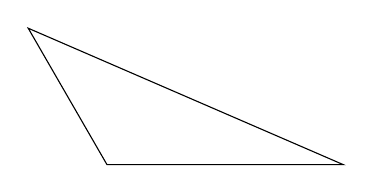
\begin{tikzpicture}
  \coordinate (A) at (0:3cm);
  \coordinate (B) at (120:2cm);

  \draw (0,0) -- (A) -- (B) -- cycle;
\end{tikzpicture}
\end{VerbatimOut}
\ShowExample

It is also possible to specify relative coordinates:
by prefixing the coordinate with \verb|++|, it is relative to the previous position.%
\footnote{It is also possible to prefix with just \texttt{+},
in which case the current position is not updated.}
%
\begin{VerbatimOut}{\jobname.tmp}
\begin{tikzpicture}
  \draw (0,0) -- ++(0:3) -- ++(90:2)
    -- ++(180:1) -- ++(270:1/2);
\end{tikzpicture}
\end{VerbatimOut}
\ShowExample


%
%
\subsection{Nodes}

Nodes can be thought of as text placed in the picture.
The text can contain mathematics and formatting commands, and even pictures.

A node can be placed either as part of a path, or separately with a \cmd{node} command.
In the latter case, it is possible to refer to the node later.
%
\begin{VerbatimOut}{\jobname.tmp}
\begin{tikzpicture}
  \draw (0,0) -- (2,0) node {Left};
  \node (A) at (0,2) {Above};
  \draw (0,0) -- (A);
  \node at (0,-1) {Below};
\end{tikzpicture}
\end{VerbatimOut}
\ShowExample

Note the difference between the lines connecting the origin to the Left and Above nodes.
When a node is created as part of a path operation,
it is \emph{centered} at the specified coordinate.
That is, the center of the ``Left'' text is at $(2,0)$.
The position of the node can be customized by passing
\verb|above|, \verb|below|, \verb|left|, or \verb|right| as an optional argument.

On the other hand, when a path is drawn to a previously defined node,
TikZ tries to stop at the boundary of the node.
It is possible to specify the position on the border by cardinal directions (like \verb|north|)
or an angle; or to specify \verb|center| if you really mean the center.
These are given by the \verb|name.anchor| syntax as in the example below.

To make the boundary of the ``Above'' node visible,
we also pass the \verb|draw| option to the \cmd{node} command.
%
\begin{VerbatimOut}{\jobname.tmp}
\begin{tikzpicture}
  \draw (0,0) -- (2,0) node[right] {Left};
  \node[draw] (A) at (0,2) {Above};
  \draw (0,0) -- (A.west);
\end{tikzpicture}
\end{VerbatimOut}
\ShowExample

One more interesting positioning specifier is the optional \verb|pos| argument.
It is understood as a position (in the range 0 to 1) on the previous path segment.
It can be combined with other specifiers as in here:
%
\begin{VerbatimOut}{\jobname.tmp}
\begin{tikzpicture}
  \draw[->] (0,0) -- (3,0)
    node[pos=0.5,above] {$\frac 1 2$}
    node[pos=0.25,below] {$\frac 1 4$}
    node[pos=0.75,below] {$\frac 3 4$};
\end{tikzpicture}
\end{VerbatimOut}
\ShowExample

To embed pictures,
you can use \cmd[in TikZ]{includegraphics} as usual inside a node.
To illustrate this once more with our fur-shedding assistants:
%
\begin{VerbatimOut}{\jobname.tmp}
\centering
\newcommand{\dogfile}{pictures/TheDogs.jpg}
\begin{tikzpicture}
  \node[draw] (Both) at (0,0)
    {\includegraphics[height=3cm]{\dogfile}};
  \node[draw] (Netta) at (-5,0)
    {\includegraphics[bb=1cm 2cm 3cm 5cm, clip, height=2cm]{\dogfile}};
  \node[draw] (Cira) at (5,0)
    {\includegraphics[bb=2.8cm 1.4cm 7cm 6cm, clip, height=2cm]{\dogfile}};
  \draw[->] (Both.west) -- (Netta.east) node[pos=0.5, above] {Netta};
  \draw[->] (Both.east) -- (Cira.west) node[pos=0.5, above] {Cira};
\end{tikzpicture}
\end{VerbatimOut}
\ShowExampleBelow[2]


%
%
\subsection{Path options}

There are lots of options that can be passed to the drawing commands.
As the very first one, let us consider \verb|color|.
It takes a colour name as its argument;
\pkg[with TikZ]{xcolor} extensions and custom colours are supported.
It is possible to blend the color with white with the \verb|!| specifier
(see page~\pageref{ex:color blending}).
Be careful with the colour name; the error message can be confusing.
%
\begin{VerbatimOut}{\jobname.tmp}
\definecolor{Sciency}{cmyk}{0,0.46,1,0}
\begin{tikzpicture}
  \draw[color=blue] (0,0)--++(3,0);
  \draw[color=LimeGreen] (0,-0.5)--++(3,0);
  \draw[color=Sciency] (0,-1)--++(3,0);
  \draw[color=Sciency!60] (0,-1.5)--++(3,0);
\end{tikzpicture}
\end{VerbatimOut}
\ShowExample

There is also a range of line weights.
Do note that their names may include spaces.
Of these, \verb|thin| is the default.
%
\begin{VerbatimOut}{\jobname.tmp}
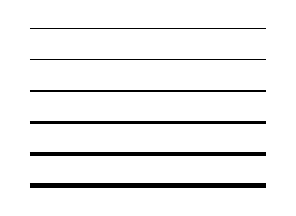
\begin{tikzpicture}[yscale=0.8]
  \draw[very thin] (0,-0.5)--++(3,0);
  \draw[thin] (0,-1)--++(3,0);
  \draw[semithick] (0,-1.5)--++(3,0);
  \draw[thick] (0,-2)--++(3,0);
  \draw[very thick] (0,-2.5)--++(3,0);
  \draw[ultra thick] (0,-3)--++(3,0);
\end{tikzpicture}
\end{VerbatimOut}
\ShowExample

Then, there are the line styles.
The basic ones are (it is possible to specify custom ones, but that you have to read from the docs):
%
\begin{VerbatimOut}{\jobname.tmp}
\begin{tikzpicture}[yscale=0.8]
  \draw[solid] (0,0.5)--++(3,0);
  \draw[dashed] (0,-0)--++(3,0);
  \draw[dotted] (0,-0.5)--++(3,0);
  \draw[densely dashed] (0,-1)--++(3,0);
  \draw[densely dotted] (0,-1.5)--++(3,0);
  \draw[loosely dashed] (0,-2)--++(3,0);
  \draw[loosely dotted] (0,-2.5)--++(3,0);
  \draw[dash dot] (0,-3)--++(3,0);
  \draw[dash dot dot] (0,-3.5)--++(3,0);
\end{tikzpicture}
\end{VerbatimOut}
\ShowExample

\begin{practices}
As remarked in the section on colour,
you should never use colour as the sole means of giving information.
In simple line graphics, the combination of colour and line style is often useful.
However, complex line styles are also hard to read!
\end{practices}


Finally, there are the arrows.
The syntax for arrow tips is $\langle\textit{start}\rangle$\verb|-|$\langle\textit{end}\rangle$,
where the start/end specification can contain one or more \verb|<|, \verb|>|, or \verb$|$.
%
\begin{VerbatimOut}{\jobname.tmp}
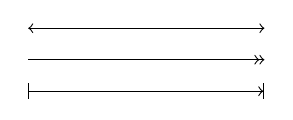
\begin{tikzpicture}[yscale=0.8]
  \draw[<->] (0,-0)--++(3,0);
  \draw[->>] (0,-0.5)--++(3,0);
  \draw[|->|] (0,-1.0)--++(3,0);
\end{tikzpicture}
\end{VerbatimOut}
\ShowExample
%
The \verb|arrows.meta| extension library contains many more tip styles
and options to customize their size; see \cite[Section~16]{tikz}.
%
\begin{VerbatimOut}{\jobname.tmp}
% \usetikzlibrary{arrows.meta}
\begin{tikzpicture}[yscale=0.8]
  \draw[Circle-{Circle[open]}] (0,-0)--++(3,0);
  \draw[-{Stealth[length=5mm,width=2mm,red]}] (4,0)--++(3,0);
  \draw[{->[harpoon]}] (8,0)--++(3,0);
\end{tikzpicture}
\end{VerbatimOut}
\ShowExampleBelow

One more option: the \verb|rounded corners| option does what is says.
It takes as its argument a radius of the corner.
It is one of the few options that can be changed in the middle of a path
(none of the above can, unfortunately).
%
\begin{VerbatimOut}{\jobname.tmp}
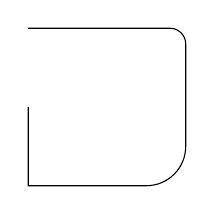
\begin{tikzpicture}
  \draw[rounded corners=2mm] (0,0) -- (2,0)
    [rounded corners=5mm] -- (2,-2)
    [sharp corners] -- (0,-2) -- (0,-1);
\end{tikzpicture}
\end{VerbatimOut}
\ShowExample



%
%
%
\section{Special paths}

In addition to the \verb|--| style path joining two points,
there are the \verb$|-$ and \verb$-|$ styles.
These split the line into vertical and horizontal segments,
the order of which you can probably guess.
%
\begin{VerbatimOut}{\jobname.tmp}
\begin{tikzpicture}
  \draw (0,0) -| (2,1);
\end{tikzpicture}
\end{VerbatimOut}
\ShowExample

To draw rectangles, there is the \verb|rectangle| shorthand
that is put between coordinates of the two opposite corners.
Similarly, there is the \verb|circle| command that is put after the centre coordinate
and takes the radius as an optional parameter.
It is possible to specify \verb|x radius| and \verb|y radius| separately to get an ellipse
(which can be further rotated with the \verb|rotate| parameter).

Moreover, the command \cmd{fill} does exactly what you would expect it to;
it fills the enclosed region.
The combination \cmd{filldraw} both fills and draws.
If you have defined the path through line segments,
the path is automatically closed.%
\footnote{If the lines cross, the definition of interior can be customized with optional arguments
\texttt{nonzero rule} and \texttt{even odd rule}.
These are defined in \cite[Section~15.5.2]{tikz}.}
%
\begin{VerbatimOut}{\jobname.tmp}
\centering
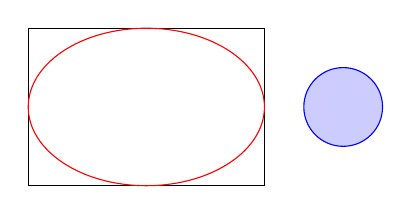
\begin{tikzpicture}
  \draw (0,0) rectangle (3,2);
  \draw[red] (3/2,1) circle
    [x radius=3/2, y radius=1];
  \filldraw[blue, fill=blue!20] (4,1) circle [radius=0.5];
\end{tikzpicture}
\end{VerbatimOut}
\ShowExampleBelow[2]

There are also commands for drawing arcs, parabolas, and even Bézier curves;
see \cite[Section~14]{tikz}.

There is a helper command for drawing coordinate grids.
TikZ provides a shorthand style \verb|help lines|
that can be customized as in \Cref{sec:tikz styles}.
Here we overlay two grids with different step sizes (default is one unit).
%
\begin{VerbatimOut}{\jobname.tmp}
\centering
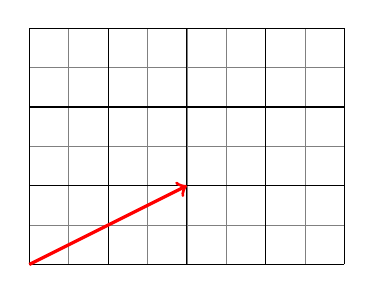
\begin{tikzpicture}
  \draw[help lines, xstep=0.5, ystep=0.5] (0,0) grid (4,3);
  \draw (0,0) grid (4,3);
  \draw[red,very thick,->] (0,0) -- (2,1);
\end{tikzpicture}
\end{VerbatimOut}
\ShowExampleBelow[2]

Now that we know how to draw a coordinate grid,
it is very natural to draw some functions on it!
TikZ includes a reasonably complex calculation engine,
which makes it possible to draw some complicated functions.
%
\begin{VerbatimOut}{\jobname.tmp}
\centering
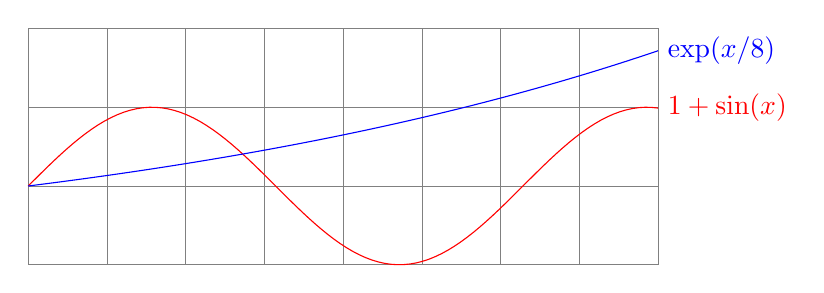
\begin{tikzpicture}
  \draw[help lines] (0,0) grid (8,3);
  \draw[red, domain=0:8, samples=100] plot (\x, {1+sin(\x r)})
    node[right] {$1+\sin(x)$};
  \draw[blue, domain=0:8, samples=100] plot (\x, {exp(\x/8)})
    node[right] {$\exp(x/8)$};
\end{tikzpicture}
\end{VerbatimOut}
\ShowExampleBelow[2]
Some notes on the usage:
\begin{itemize}
\item The domain is specified using the syntax \verb|lower:upper|.
\item The number of samples is optional to specify, but the default value is quite small.
\item The variable $x$ is written with a backslash \verb|\x|,
    but the mathematical commands are spelled without a backslash.
\item Mathematical expressions should be wrapped inside \verb|{}|.
\item Trigonometric functions assume degrees by default;
    the suffix \verb|r| after \verb|\x| converts the variable into radians.
\end{itemize}

Note that the plot is still defined as a pair of $(x,y)$ coordinates.
This makes it possible to draw parametric plots.
The name of the variable can be customized.
%
\begin{VerbatimOut}{\jobname.tmp}
\centering
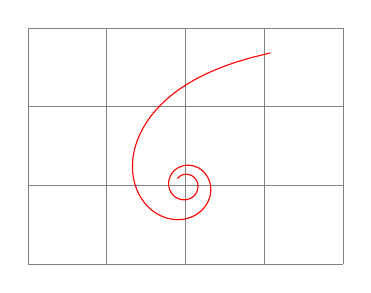
\begin{tikzpicture}
  \draw[help lines] (-2,-1) grid (2,2);
  \draw[red, domain=1:15, samples=150, variable=\t]
    plot ({2*cos(\t r) / \t}, {2*sin(\t r) / \t});
\end{tikzpicture}
\end{VerbatimOut}
\ShowExampleBelow[2]

It is also possible to plot individual points or bar graphs,
or to even load a dataset from an external file.
See \cite[Section~22]{tikz} for more,
but also note the warnings below.

\begin{warning}
``Division by zero'' and ``number too big`` errors
can sometimes lead to confusing (and repeated!) error messages.
\end{warning}

\begin{practices}
TikZ is excellent for producing small and simple function plots
in a style consistent with the rest of the document.
However, compilation times can get quite long for even slightly complicated functions.

If you need to plot lots of complex functions,
you should precompute the function values in a file
and use the data plotting facility of TikZ; see \cite[Section~22]{tikz}.
\end{practices}



%
%
\section{Transformations}

The \verb|xshift|, \verb|yshift|, \verb|rotate|, and \verb|scale| optional arguments
can be used to locally change the coordinate system.%
\footnote{There are some more; see \cite[Section~25.3]{tikz} for details.
A particular example is \texttt{rotate around}, which rotates around a specified point.}
You can use a \env{scope} environment within the picture
to pass the transformation to multiple drawing operations:
%
\begin{VerbatimOut}{\jobname.tmp}
\centering
\begin{tikzpicture}
  \draw (0,0) rectangle (2,1);
  \begin{scope}[xshift=3cm]
    \draw[dotted] (0,0) rectangle (2,1);
  \end{scope}
  \begin{scope}[xshift=6.2cm, scale=0.5, rotate=30]
    \draw[blue] (0,0) rectangle (2,1);
  \end{scope}
\end{tikzpicture}
\end{VerbatimOut}
\ShowExampleBelow[2]
%
Note that the \verb|xshift| parameter should be specified with a unit
(otherwise the unit is assumed to be \verb|pt|).
The \env{scope} environment can be used to pass any optional arguments to enclosed commands;
for example, color or line style declarations can be passed as well.

Sometimes it is necessary to extend or to shrink the bounding box of the picture.
For this, the \cmd{useasboundingbox} command is useful.%
\footnote{Let us note that this is a shorthand for
\texttt{\textbackslash{}path[use as bounding box]};
TikZ certainly has many ways to do common operations.}
(This is especially useful in a Beamer slide where you gradually reveal parts of the picture.
You can use this command to reserve enough space for the full picture.)

Here we instead shrink the bounding box
so that the picture contents extend beyond the reserved space.
The dramatic effect is somewhat ruined by displaying the bounding box.
%
\begin{VerbatimOut}{\jobname.tmp}
\centering
Then a huge seagull
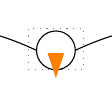
\begin{tikzpicture}
  \useasboundingbox[draw,dotted,gray] (-1em,-0.7em) rectangle (1em,0.8em);

  \draw (0,0) circle [radius=0.7em];
  \fill[orange] (-0.3em,-0.1em)--(0.3em,-0.1em)--(0em,-1em)--cycle;
  \draw (0.7em,0em) parabola bend (5em,1em) (6em,0.8em);
  \draw (-0.7em,0em) parabola bend (-5em,1em) (-6em,0.8em);
\end{tikzpicture}
came swooping down.
\end{VerbatimOut}
\ShowExampleBelow[2]



%
%
\section{Loops}

TikZ automatically loads the \pkg{pgffor} package that provides a useful \cmd{foreach} command.
It can be used in two ways.
The first is to loop over a given set:
%
\begin{VerbatimOut}{\jobname.tmp}
\centering
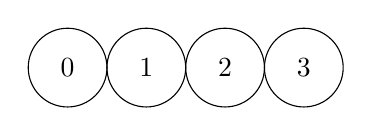
\begin{tikzpicture}
  \foreach \x in {0,1,2,3}
    \draw (\x, 0) circle [radius=0.5] node {$\x$};
\end{tikzpicture}
\end{VerbatimOut}
\ShowExampleBelow[2]
%
Loops can be nested:
%
\begin{VerbatimOut}{\jobname.tmp}
\centering
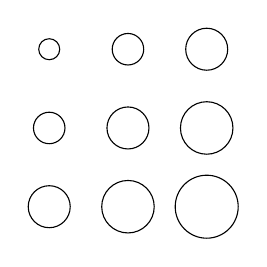
\begin{tikzpicture}
  \foreach \x in {1,2,3}
    \foreach \y in {1,2,3}
      \draw (\x, -\y) circle [radius={(\x+\y)/15}];
\end{tikzpicture}
\end{VerbatimOut}
\ShowExampleBelow[2]
With \verb|{}|, it is possible to define several commands to be executed.
It is also possible to define several variables in one loop:
%
\begin{VerbatimOut}{\jobname.tmp}
\centering
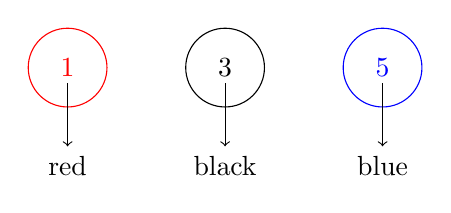
\begin{tikzpicture}
  \foreach \x/\col in {1/red, 3/black, 5/blue} {
    \draw[\col] (\x, 0) circle [radius=0.5] node {$\x$};
    \draw[->] (\x,-0.2) -- (\x,-1) node[below] {\col};
  }
\end{tikzpicture}
\end{VerbatimOut}
\ShowExampleBelow[2]

Another way to use \cmd{foreach} is to specify a range.
It takes the first, second, and last element, and \verb|...| before the final element.
%
\begin{VerbatimOut}{\jobname.tmp}
\centering
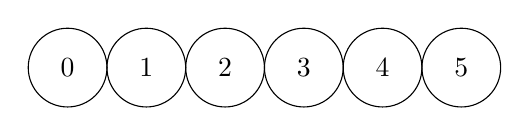
\begin{tikzpicture}
  \foreach \x in {0,1,...,5}
    \draw (\x, 0) circle [radius=0.5] node {$\x$};
\end{tikzpicture}
\end{VerbatimOut}
\ShowExampleBelow[2]

Finally, let us note that the \cmd{foreach} command can freely be used outside TikZ.
(If you do not need full TikZ, you can just load the \pkg{pgffor} package.)
%
\begin{VerbatimOut}{\jobname.tmp}
\foreach \dog/\yr in {Cira/2009, Netta/2016}
  {\dog{} was born in \yr{}.\\}
\end{VerbatimOut}
\ShowExample


%
%
\section{\emph{Setting styles*}}\label{sec:tikz styles}

In the grid example, we saw the \verb|help lines| style that produced thin, gray lines.
TikZ provides a general facility for setting up such shorthand styles.
If you find yourself repeating graphical options,
you should consider using a style instead.%
\footnote{Those familiar with web development notice that this system is similar to
Cascading Style Sheets (CSS); indeed, the TikZ style system is inspired by it.}

To customize the style,
you use the \verb|/.style={}| syntax in the optional argument to the picture environment:
%
\begin{VerbatimOut}{\jobname.tmp}
\centering
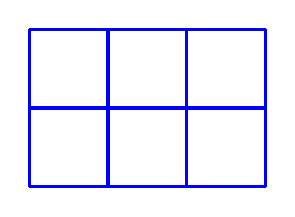
\begin{tikzpicture}[help lines/.style={very thick,blue}]
  \draw[help lines] (0,0) grid (3,2);
\end{tikzpicture}
\end{VerbatimOut}
\ShowExampleBelow[2]

If you only want to customize part of the style,
you can keep the previous elements in place by using \verb|/.append style={}| instead.
Here we keep the lines thin and gray, but also make them dashed:
%
\begin{VerbatimOut}{\jobname.tmp}
\centering
\begin{tikzpicture}[help lines/.append style={dashed}]
  \draw[help lines] (0,0) grid (3,2);
\end{tikzpicture}
\end{VerbatimOut}
\ShowExampleBelow[2]

You can define your own styles with the \verb|/.style| syntax.
To reuse them across multiple TikZ environments,
you can put the definition in a \cmd{tikzset} command.
Such a command could go into the preamble.
It is still possible to override styles locally.
Here we define a style called \verb|highlight|:
%
\begin{VerbatimOut}{\jobname.tmp}
\centering
\tikzset{highlight/.style={draw,very thick,orange}}
\newcommand{\dogfile}{pictures/TheDogs.jpg}

\begin{tikzpicture}
  \node[highlight] at (-2,0)
    {\includegraphics[bb=1cm 2cm 3cm 5cm, clip, height=2cm]{\dogfile}};
  \node[highlight, blue] at (2,0)
    {\includegraphics[bb=2.8cm 1.4cm 7cm 6cm, clip, height=2cm]{\dogfile}};
\end{tikzpicture}
\end{VerbatimOut}
\ShowExampleBelow[2]


\begin{practices}
Do note that this idea goes very well with the separation of content and presentation.
If your document contains a lot of TikZ graphics with repeated graphical styles,
you should use styles with descriptive names.
Not only is the code semantically meaningful, but also easier to change.
\end{practices}


%
%
\section{Some extensions}

TikZ comes with several extension libraries that are not loaded by default.
They can be enabled with \cmd{usetikzlibrary}.
Their full documentation fills \cite[Section~V]{tikz},
but let us briefly show some of the more useful packages.

\todo{Think about what to cover here: angles, decorations, graphs, trees, spy?}

%
\subsection{Commutative diagrams}\label{sec:tikz-cd}

In certain fields of mathematics, everything is explainable with sufficiently many arrows.
If you are one of those people, then you will love the \pkg{tikz-cd} package.
It can also be loaded through \verb|\usetikzlibrary{cd}|.
%
\begin{VerbatimOut}{\jobname.tmp}
\centering
% \usetikzlibrary{babel} % Might be needed, see below
% \usetikzlibrary{cd}

\begin{tikzcd}
A \arrow[r] \arrow[d, dotted] & B \arrow[d, Rightarrow, bend left]\\
C \arrow[r, maps to, "\psi"]  & D
\end{tikzcd}
\end{VerbatimOut}
\ShowExampleBelow[2]

\begin{gotcha}
If you get an error message when you try to add a label (like \verb|"\psi"| above),
you should try loading the \verb|babel| TikZ library.
This relates to the handling of quotation marks by \pkg[TikZ compatibility]{babel} package;
the TikZ support library fixes up the handling inside TikZ environments.
\end{gotcha}

There is a nice online editor for commutative diagrams by Yichuan Shen.%
\footnote{\url{https://tikzcd.yichuanshen.de/}}
It only supports a subset of \pkg{tikz-cd} features,
but is a nice and visual way to edit the diagram before exporting its \LaTeX{} code.
(It also supports \emph{importing} code for further editing!)

% !TeX root = 2nd-course-in-latex.tex
\chapter{Presentations with Beamer}

If you ask me, Beamer is an odd tool.
Presentations are inherently visual,
so a programming tool like \LaTeX{} seems ill-suited for the job.
On the other hand, most graphical programs cannot match the quality of \LaTeX{} mathematics,
and technical talks often have modest visual needs.

Beamer does strike a nice balance between the two,
if only your talk is not too ambitious with the visuals.
At the same time I find its complexity to be similar to TikZ
-- a lot of things are possible, but not all of them are advisable.

\begin{practices}
Even though this course is not about presentation skills,
I want to use this opportunity for an important reminder:
Beamer makes it very easy to throw too much mathematics at your audience.

Leave whitespace on your slides, and focus on pictures to support your point.
If you want to dive deep into a mathematical topic,
there is an even superior tool: blackboard.
\end{practices}


%
%
\section{Basic structure}

Beamer is implemented as the \textbf{beamer} document class.
A minimal Beamer file is thus:
%
\begin{ExampleCode}
\documentclass{beamer}

\begin{document}

\begin{frame}
\end{frame}

\end{document}
\end{ExampleCode}
%
Beamer automatically loads \pkg[Beamer]{hyperref}.
It also loads \pkg[Beamer]{amsthm} and creates some theorem environments by default.

Since \TeX{} always believes it is typesetting for printing,
Beamer modifies the page size to be suitable.
By default it is $128 \times 96$~mm, which corresponds to 4:3 aspect ratio.

To modify the aspect ratio, you can pass the \verb|aspectratio| class option.
It is a string of two to four digits, and interpreted like:
\verb|aspectratio=32| means 3:2, \verb|169| means 16:9, and \verb|1610| means 16:10.

\begin{practices}
Many computer screens have 16:9 or 16:10 aspect ratio, so 4:3 might seem old-fashioned.
However, 4:3 has the benefit of increased vertical space.
Many projectors can output either aspect ratio comfortably.
If possible, check the venue beforehand.
\end{practices}

The default 11~pt font fits very nicely with the simulated paper size.
You can pass the \verb|10pt| or \verb|12pt| class options to modify the font size a bit.%
\footnote{There are also some more choices,
but they make the text either very large of very unreadable.}

\begin{gotcha}
You should put \verb|\usefonttheme{professionalfonts}| in the preamble
if you use \mbox{LuaTeX} or XeTeX.
It appears that Beamer does not always recognize that Latin Modern is in use with these compilers.
If the font theme is not changed,
Beamer might produce bad kerning for some specific letter combinations.
\end{gotcha}


For basic title design, you can use the usual \cmd{title}, \cmd{author}, and \cmd{date} commands.
There is also an \cmd{institute} command for specifying the author institution,
and a \cmd{titlegraphic} command that can be used for a logo etc.
Thus a basic presentation with just a title page is set with:
%
\begin{ExampleCode}
\title{My fantastic presentation}
\author{Firstname Lastname}
\institute{University of Puuhamaa}
\titlegraphic{\includegraphics[width=3cm]{TheDogs.jpg}}
\date{20 May 2024}

\begin{document}

\maketitle

\end{document}
\end{ExampleCode}
%
\EmbedPdfPage{examples/basic-beamer.pdf}{1}
%
(The \cmd{maketitle} command can be inside or outside a \verb|frame| environment.
The command is synonymous with \cmd{titlepage}.)

New slides are created with the \env{frame} environments.
Each slide acts like a page, so the basic typesetting commands are available.
The title for the frame can be set with \cmd{frametitle};
it is displayed in the frame header.
%
\begin{ExampleCode}
\begin{frame}
\frametitle{Hi there!}

Welcome to my presentation!

We will talk about Pythagoras and his theorem.
\end{frame}
\end{ExampleCode}
%
\EmbedPdfPage{examples/basic-beamer.pdf}{2}

Note that the paragraphs have no visual separation whatsoever.
You can of course set \cmd[Beamer]{parskip} to a better value
(I suggest a larger value than for printed documents, like 1~em),
but Beamer presentations are often composed of \emph{blocks}.
The \env{block} environment has a title and content:
%
\begin{ExampleCode}
\begin{frame}
\frametitle{Hi there!}

Welcome to my presentation!

\begin{block}{Goal}
You will learn about Pythagoras and his theorem.
\end{block}
\end{frame}
\end{ExampleCode}
%
\EmbedPdfPage{examples/basic-beamer.pdf}{3}
%
In this example the block is not very highlighted,
but that can be changed with a suitable colour theme.
We'll get to that in \Cref{sec:beamer styles}.

By default, Beamer creates a few common theorem environments.
More can be created with the usual \pkg[Beamer]{amsthm} commands (see \Cref{sec:amsthm}).
%
\begin{ExampleCode}
\begin{frame}
\frametitle{The theorem}

\begin{theorem}
If $a$ and $b$ are the lengths of catheti of a right-angled triangle,
then the hypothenuse has length $\sqrt{a^2 + b^2}$.
\end{theorem}
\begin{proof}
We'll get to this soon.
\end{proof}

\end{frame}
\end{ExampleCode}
%
\EmbedPdfPage{examples/basic-beamer.pdf}{4}


To highlight text, it is advisable to use the \cmd{alert} command.
By default it makes the text red, but the style can be customized.

The usual list environments can be used.
Beamer loads the \pkg{enumerate} package that enables a shorthand styling syntax
for \env[shorthand styles]{enumerate} environments.

Let us illustrate these elements with a multi-column layout.
Such a layout is created with a \env[Beamer]{columns} environment.
It takes an optional vertical alignment specifier (top by default;
vertical centres with \verb|c| and bottoms by \verb|b|).%
\footnote{If things do not align as you would expect,
you should also try the \texttt{T} option:
it aligns baselines of the first lines instead of tops of lines.}
%
Inside this environment, columns are created with the \env[Beamer]{column} environment,
which takes column width as a required argument.%
\footnote{There is also an equivalently named command
if you prefer to avoid deeply nested environments.}
%
\begin{ExampleCode}
\begin{columns}
\begin{column}{0.5\textwidth}

Properties of \alert{Pythagoras}:
\begin{enumerate}[1.]
    \item From Ancient Greece ...
\end{enumerate}
\end{column}

\begin{column}{0.5\textwidth}
Properties of \alert{the theorem}:
\begin{enumerate}[i)]
    \item Not invented by Pythagoras ...
\end{enumerate}

\end{column}
\end{columns}
\end{ExampleCode}
%
\EmbedPdfPage{examples/basic-beamer.pdf}{5}


\begin{gotcha}
Frames do not really support the \env[Beamer]{verbatim} environment;
the \pkg{listings} package is probably visually nicer anyways.
\end{gotcha}


%
%
\section{Including graphics}

The usual graphics commands of \LaTeX{} and TikZ can be used as usual.
Moreover, the usual \env[Beamer]{figure} and \env[Beamer]{table} environments can be used.
%
\begin{ExampleCode}
\begin{figure}
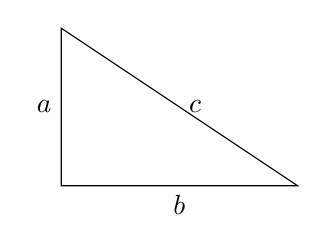
\begin{tikzpicture}
    \draw (0,0) -- (0,2) node[pos=0.5, left] {$a$}
        -- (3,0) node[pos=0.5, right] {$c$}
        -- cycle node[pos=0.5, below] {$b$};
\end{tikzpicture}
\caption{A right triangle.}
\end{figure}

\begin{figure}
    \includegraphics[width=3cm]{TheDogs.jpg}
\caption{Slide hijacked by a dog!}
\end{figure}
\end{ExampleCode}
%
\EmbedPdfPage{examples/basic-beamer.pdf}{6}

\begin{gotcha}
As with article classes, figures are not placed side by side.
The \pkg{subcaption} package is again useful for that;
see \Cref{sec:subfigures}.
Moreover, there is no automatic page breaking:
if you put too much stuff on a slide, they will overflow.
\end{gotcha}


\todo{Absolute positioning}


\begin{warning}
You can find code examples and Beamer documentation about embedding video files inside a presentation.
This is a great way to make a presentation work only on a specific Acrobat Reader version
and only on your current computer.
It is 99~\% guaranteed not to work at a conference venue.

As annoying as it is to switch between programs to show videos,
it is the only reliable option.
\end{warning}



%
%
\section{Uncovering things}

The easiest way to uncover things piecewise is the \cmd{pause} command.
As the name suggests, it inserts a slide break at the source location.
%
\begin{ExampleCode}
\begin{frame}
\frametitle{A digression on numbers}

\begin{theorem}
Every natural number has a successor.
\end{theorem}

\pause

\begin{theorem}
There is at least one natural number.
\end{theorem}

\pause

\begin{corollary}
There are infinitely many natural numbers.
\end{corollary}
\end{frame}
\end{ExampleCode}
%
\begin{center}
\fbox{\includegraphics[page=7, width=0.3\textwidth]{examples/basic-beamer.pdf}}~
\fbox{\includegraphics[page=8, width=0.3\textwidth]{examples/basic-beamer.pdf}}~
\fbox{\includegraphics[page=9, width=0.3\textwidth]{examples/basic-beamer.pdf}}
\end{center}

The \cmd{pause} command can be used in many places:
between blocks and paragraphs and inside lists.

\begin{gotcha}
The \cmd{pause} command does not work inside \pkg[with Beamer]{amsmath} environments.
\todo{Workarounds?}
\end{gotcha}

To get more control, it is possible to use the \cmd{uncover} command
and \emph{overlay specifications}.
Here are some example overlay specifications:
\begin{description}
\item[\texttt{<2>}] Only shown on slide~2.
\item[\texttt{<2->}] Shown on slide~2 and all following slides.
\item[\texttt{<2-3,5>}] Shown on slides~2--3 and~5.
\end{description}
%
The block environments support overlay specifications,
so the previous example could be rewritten as:
%
\begin{ExampleCode}
\begin{frame}
\frametitle{A digression on numbers, version 2}

\begin{theorem}<1->
Every natural number has a successor.
\end{theorem}

\begin{theorem}<2->
There is at least one natural number.
\end{theorem}

\begin{corollary}<3->
There are infinitely many natural numbers.
\end{corollary}
\end{frame}
\end{ExampleCode}
%
There is also a shorthand syntax \verb|<+->| that is functionally similar to \cmd{pause}:
it increments the previous overlay specification by one.%
\footnote{To be precise, the magic command is \texttt{+}:
it is replaced by the previous slide number, and the slide number is then incremented.}
In the previous example, all overlay specifications could be replaced by \verb|<+->|.
This is particularly useful for lists:
%
\begin{ExampleCode}
\begin{itemize}
    \item<+-> This is shown starting from the first slide.
    \item<+-> This is shown starting from the second slide.
    \item<+-> This is shown starting from the third slide.
\end{itemize}
\end{ExampleCode}
%
Beamer introduces an optional argument to produce such lists with even less repetition:
%
\begin{ExampleCode}
\begin{itemize}[<+->]
    \item This is shown starting from the first slide.
    \item This is shown starting from the second slide.
    \item This is shown starting from the third slide.
\end{itemize}
\end{ExampleCode}

Outside an environment or list, the \cmd{uncover} command works the same:
%
\begin{ExampleCode}
\begin{frame}
\frametitle{On the infinitude of numbers}

\begin{corollary}
There are infinitely many natural numbers.
\end{corollary}
\begin{proof}
\uncover<2->{Suppose that $n$ is the largest natural number.}
\uncover<3->{But then its successor $n+1$ is an even larger natural number.}
\end{proof}

\end{frame}
\end{ExampleCode}
%
\begin{center}
\fbox{\includegraphics[page=10, width=0.3\textwidth]{examples/basic-beamer.pdf}}~
\fbox{\includegraphics[page=11, width=0.3\textwidth]{examples/basic-beamer.pdf}}~
\fbox{\includegraphics[page=12, width=0.3\textwidth]{examples/basic-beamer.pdf}}
\end{center}

Overlay specifications can also be applied to text styling commands like \cmd{alert}.
In this case, the text styling is only applied on the specified frames.
%
\begin{ExampleCode}
\begin{frame}

\textbf<1>{Bold on the first slide only.}\\
\alert<2>{Alerted on the second slide only.}

\end{frame}
\end{ExampleCode}
%
\begin{center}
\fbox{\includegraphics[page=13, width=0.45\textwidth]{examples/basic-beamer.pdf}}~
\fbox{\includegraphics[page=14, width=0.45\textwidth]{examples/basic-beamer.pdf}}
\end{center}

\todo{Alert shorthand for lists, \texttt{<.>}?}

There is also an \cmd{only} command.
Its difference to the \cmd{uncover} command is that no space is reserved.
Since it may cause the positioning of the adjacent text change
between slides, it should only be used when necessary.
%
\begin{ExampleCode}
\begin{frame}

There is nothing to see here.\\
\only<2>{\includegraphics[width=6cm]{../pictures/TheDogs.jpg}\\}
Absolutely nothing at all.

\end{frame}
\end{ExampleCode}
%
\begin{center}
\fbox{\includegraphics[page=15, width=0.45\textwidth]{examples/basic-beamer.pdf}}~
\fbox{\includegraphics[page=16, width=0.45\textwidth]{examples/basic-beamer.pdf}}
\end{center}

\todo{reserving space}

\todo{againframe}


%
%
\section{Sections and parts}

\todo{Section and part commands}

\todo{Appendices}

\todo{Tables of contents}

\todo{Bibliography}


%
%
\section{Styling it}\label{sec:beamer styles}

\todo{Navigation symbols, advanced typography}

\todo{Transparency in uncovering}

\todo{The templating system}

\begin{technote}
As with embedded videos, it is possible to specify slide transition effects,
but they might not work with all PDF viewers.
Because of this, we do not discuss them here.
\end{technote}

\subsection{Themes}
\todo{Outline of the theme system}

\subsection{Colours}
\todo{fg and bg colors, using and setting them}

\subsection{Fonts}
\todo{Fonts}


%
%
\section{Handouts}

\todo{About this mode; also mention multiple slides per sheet (21.1)}

\todo{Overlay specifications}

\chapter{Posters with tikzposter}

There are several methods to creating posters with \LaTeX{}.
To mention just three of the many packages: \pkg{tikzposter}, \pkg{beamerposter}, and \pkg{tcolorbox}.
All of them suffer from the fact that posters are very visual,
but \TeX{} can really only do boxes.

Here we discuss \pkg{tikzposter} since it is reasonably simple.
However, the package has not been actively maintained since~2014,
and it appears to have some bugs.
The other packages use fairly similar principles.

\begin{remark}
In particular, I would like to highlight \pkg{tcolorbox} for its good documentation.
You should definitely check it out.

Note that its poster template does not handle large paper sizes.
You can either configure the paper and font sizes by yourself,
or scale up the A3-size output in the printing phase.
The latter may be frowned upon by typography enthusiasts,
since a 12-point font scaled 4$\times$ is \emph{very much not the same} as a 48-point font.
\end{remark}


%
%
\section{Basic layout}

The package is loaded with
%
\begin{ExampleCode}
\documentclass{tikzposter}
\end{ExampleCode}
%
By default, the options \verb|a0paper|, \verb|25pt|, and \verb|portrait| are used.
Paper sizes A1 and A2 are also available, and the \verb|landscape| option produces a landscape page.
The range of font sizes is limited to 12, 14, 17, 20, and 25~points.
Of these, only the last one is suitable for A0~size.

\begin{practices}
As with presentations, you should not have too much text.
Use whitespace and structure to guide the reader.
\end{practices}

For one reason or other, the package adds a watermark to the lower-right corner.
It can be turned off with the monstrously long command
%
\begin{ExampleCode}
\tikzposterlatexaffectionproofoff
\end{ExampleCode}
%
There are also some package options to control margins and default block spacing;
see the documentation for details.

The title is set with \cmd[tikzposter]{maketitle} as usual;
you can set \cmd{title}, \cmd{author}, and \cmd{institute} in the preamble.
You can also put graphical (or rather, any) commands inside \cmd{titlegraphic}.
By default these elements are set on top of each other.
The customization is briefly discussed in \Cref{sec:poster style}.
The \cmd[tikzposter]{maketitle} command also accepts some optional arguments like
%
\begin{ExampleCode}
\maketitle[width=40cm]
\end{ExampleCode}



As with Beamer, the basic layout consists of blocks.
The \cmd[tikzposter]{block} command takes optional customization arguments,
a title, and the contents:
%
\begin{ExampleCode}
\block[]{Block title goes here}
{
Contents of the block
}
\end{ExampleCode}
%
The block will fill the available horizontal space,
and the vertical size depends on the contents.
Contents can be any material (except floats).
If the title is empty, the ``block header'' disappears.

To set several blocks side by side, it is possible to use columns
specified inside a \env[tikzposter]{columns} environment.
A new column is started with the \cmd[tikzposter]{column} command.
As its argument it takes the fraction of text area width.%
\footnote{You need to ensure that they sum to at most $1$.
The documentation also talks about absolute widths, but they do not seem to actually work.}
Any blocks specified after this command will be placed vertically in the column.
For example, here we set two columns of equal size,
and place two blocks in the left column:
%
\begin{ExampleCode}
\begin{columns}

\column{0.5}
\block{Above left}{}
\block{Below left}{}

\column{0.5}
\block{Right}{}

\end{columns}
\end{ExampleCode}

The \env[tikzposter]{subcolumns} and \cmd[tikzposter]{subcolumn}
can be used to further divide a column
(the arguments are fractions of the \emph{outer column} width).

After the \env{columns} environment ends,
all new blocks again fill the whole horizontal space.

You cannot use the usual vertical spacing commands to adjust spacing between blocks.
A workaround is to add an offset both to the block title and contents.
Negative $y$ values point downwards.%
\footnote{It appears that this method might not work with blocks without title;
this seems to be a bug.}
%
\begin{ExampleCode}
\block[titleoffsety=-2cm, bodyoffsety=-2cm]{Title}{Contents}
\end{ExampleCode}

Inside a block, you can use the \cmd[tikzposter]{coloredbox} command to create highlighted regions.
%
\begin{ExampleCode}
\block{Goal}
{
In this poster we discuss Pythagoras' theorem.

\coloredbox{It is maybe the most important theorem in human history!!}

\coloredbox[bgcolor=PeachPuff, fgcolor=red]{\centering I mean it!!!}
}
\end{ExampleCode}
%
It is also possible to add small notes.
They are defined outside blocks, but they attach to the previous block.
By default, they connect to the center of the block,
but the precise point can be adjusted with optional arguments,
as with the distance and angle (here east-southeast) to the anchor point:
%
\begin{ExampleCode}
\note[angle=-20, radius=8cm, connection, targetoffsety=-2cm]
    {This poster will convince you about it!}
\end{ExampleCode}

Let us see how these pieces (and a few more content additions) play together.
The output of the following code is shown in \Cref{fig:poster example}.

\begin{figure}
\centering
\includegraphics[height=0.85\textheight]{examples/tikzposter-content.pdf}
\caption{The example poster (set in A2 size, and scaled here).}\label{fig:poster example}
\end{figure}

\VerbatimInput[fontsize=\footnotesize,frame=lines]{examples/tikzposter-content.tex}




%
%
\section{Styling}\label{sec:poster style}

The styling system of \pkg[styling]{tikzposter} is very similar to that of Beamer.
There are a few built-in styles.%
\footnote{\url{bitbucket.org/surmann/tikzposter/downloads/styleguide.pdf}}


\begin{technote}
The source code for the predefined styles is very readable.
If you want to customize styles, I recommend using their code as a starting point.

The installation location of packages depends on your specific \LaTeX{} installation,
but the code can also be browsed online at \url{bitbucket.org/surmann/tikzposter/}.
\end{technote}


The overall look is controlled by \cmd[tikzposter]{usetheme},
and then e.g.\ the colour and background styles can be customized.
Individual colours can be changed with \cmd[tikzposter]{colorlet}
(unlike in Beamer, colours are not separated into foreground and background colours).

For example, this code selects the theme in \Cref{fig:poster styled}:
\begin{ExampleCode}
\usetheme{Envelope} % Block and title style set by this
\usecolorstyle{Denmark} % Red-white colour scheme

\usebackgroundstyle{VerticalGradation} % Vertical gradient...
\colorlet{backgroundcolor}{blue!40} % ...with a faint blue colour
\end{ExampleCode}

To modify the layout of the title contents,
it is unfortunately necessary to go to low-level \LaTeX{} code.
The \cmd[tikzposter]{settitle} command can be used to define the layout code for the title contents.
The variables set by the \verb|\maketitle| companion commands can be used as below.
The following code is also used in \Cref{fig:poster styled}:
%
\begin{ExampleCode}
\settitle{
    \makebox[6cm][c]{\@titlegraphic}
    \parbox[b]{22cm}{
        \color{titlefgcolor} {\bfseries \Huge \@title \par}
        \vspace*{1em}
        {\huge \@author{} \Large (\@institute)}
    }
}
\end{ExampleCode}

\begin{figure}
\centering
\includegraphics[height=0.85\textheight]{examples/tikzposter-style.pdf}
\caption{A styled version of the previous example.}\label{fig:poster styled}
\end{figure}

\begin{technote}
It appears that \verb|\title| as defined by the package
does not permit automatic line breaking of the title.
\end{technote}



\printindex

\end{document}
